\makeatletter
\def\@makechapterhead#1{%
  \vspace*{10\p@}%
  {\parindent \z@ \raggedleft \normalfont
    \ifnum \c@secnumdepth >\m@ne
      \if@mainmatter
        \LARGE\bfseries \@chapapp\space \thechapter
	\vskip 4pt
        \hrule height 2pt
        \par\nobreak
        \vskip 5\p@
      \fi
    \fi
    \interlinepenalty\@M
    \huge \bfseries #1\par\nobreak
\vskip 5pt

\hrule height 2pt   
 \vskip 10\p@  
  }}
\makeatother

\setcounter{chapter}{3}
\chapter{Operational Amplifiers}\label{chap4}
\addtocontents{toc}{\protect\contentsline{chapter}{\protect Chapter \numberline{\thechapter.}
  Operational Amplifiers}{\thepage--\pageref{4end}}}  

\section{Introduction}\label{sec4.1}

An operational amplifier is a very high gain directly coupled negative feedback amplifier which can amplify signals having wide range of frequencies. It was originally designed for performing mathematical operations such as addition, subtraction, multiplication, integration etc. Hence the name {\em operational amplifier} or {\em OPAMP}. But with the addition of suitable external feedback components, the modern day opamp can be used for a variety of applications such as signal amplification, filters, oscillators, regulators, comparators  etc.

\smallskip
\itheading{Schematic Symbol~:}
\begin{figure}[H]
\centering
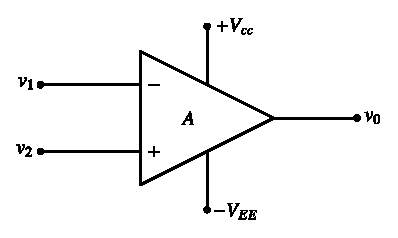
\includegraphics{chap4/fig4.1.eps}
\caption{Schematic symbol for an opamp}\label{fig4.1}
\end{figure}

Fig.~\ref{fig4.1} shows the schematic symbol for an opamp. It has 2 inputs and an output terminal. The input with `+' sign is called {\em non-inverting terminal} and that with `$-$' sign is called {\em inverting terminal}. The output voltage $v_{\rmo}$ is in-phase with the input if the signal is connected to the non-inverting terminal and $v_{\rmo}$ is out of phase with the input if the signal is connected to the inverting terminal. +V$_{\text{CC}}$ and $-$V$_{\text{EE}}$ are dc power terminals. `A' indicates the open-loop voltage gain.

\smallskip
Opamps are available in three packages :
\begin{itemize}
\item[(i)] The dual-in-line package (DIP)

\item[(ii)] The flat package

\item[(iii)] The metal can package
\end{itemize}

\itheading{Equivalent circuit of an opamp~:}
\begin{figure}[H]
\centering
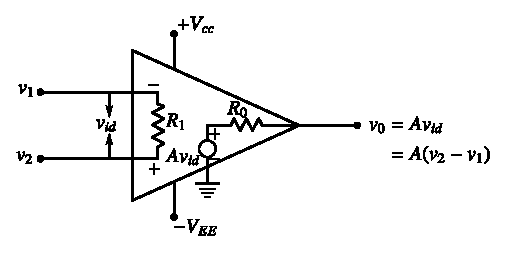
\includegraphics{chap4/fig4.2.eps}
\caption{Equivalent circuit of an opamp}\label{fig4.2}
\end{figure}

Fig.~\ref{fig4.2} shows an equivalent circuit of an opamp. The output voltage $v_{\rmo}$ is given by,
\begin{align}
\rmV_{\rmo} &= \rmA \, v_{\id}\notag\\
\text{i.e.,}\qquad \rmV_{\rmo} &= \rmA\, (v_{2}-v_{1})\label{eq4.1}
\end{align}
\begin{tabbing}
where \= $v_{\id}$ \== difference input voltage (V)\\[3pt]
      \> $v_{2}$  \>= voltage at the non-inverting terminal with respect to ground (V)\\[3pt]
      \> $v_{1}$  \>= voltage at the inverting terminal with respect to ground (V)\\[3pt]
      \> A       \>= open-loop voltage gain.
\end{tabbing}

Here $\rmA v_{\id}$ is an equivalent Thevinin's voltage source and $\rmR_{\rmo}$ is the Thevinin's equivalent resistance looking back into the output terminal of an opamp. $\rmR_{i}$ is the input resistance.

Eqn.~\eqref{eq4.1} indicates that output voltage $v_{\rmo}$ is directly proportional to the algebraic difference between the two input voltages, i.e., the opamp amplifies the difference between the two input voltages. Therefore the polarity of the output voltage depends on the polarity of the difference voltage. Eqn.~\eqref{eq4.1} is called the basic opamp equation. The graphical representation of this equation is shown in Fig.~\ref{fig4.3} where the output voltage $v_{\rmo}$ is plotted against input difference voltage $v_{\id}$, keeping A as constant.

Note that the output voltage $v_{\rmo}$ cannot exceed the +ve and $-$ve saturation voltages +V$_{\text{CC}}$ and $-$V$_{\text{EE}}$ respectively. Therefore the output voltage $v_{\rmo}$ is directly proportional to the input difference voltage $v_{2}$, until it reaches the saturation voltages and thereafter it remains constant as shown in the Fig.~\ref{fig4.3}. the graph shown is called an {\em ideal voltage transfer curve}. Since open-loop gain A is very large, a small difference input voltage $v_{\id}$ will cause the opamp output voltage $v_{\rmo}$ to be driven all the way to its extreme +ve or $-$ve V$_{\text{sat}}$.
\begin{figure}[H]
\centering
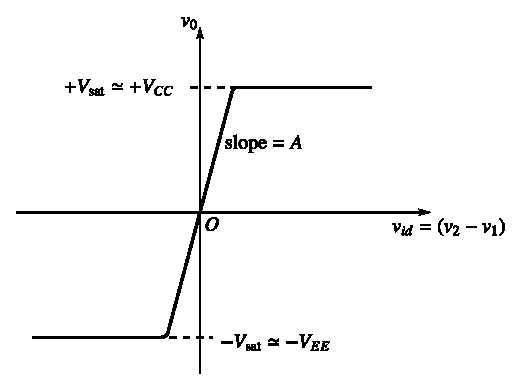
\includegraphics{chap4/fig4.3.eps}
\caption{Ideal voltage transfer curve of an opamp}\label{fig4.3}
\end{figure}

\medskip
\noindent
{\bf Note~:} From Fig.~\ref{fig4.2}, we have
\begin{align*}
v_{\rmo} &=\rmA v_{\id}\\[4pt]
 &= \rmA (v_{2}-v_{1})\\[4pt]
v_{2}-v_{1} &= \frac{\rmV_{\rmo}}{\rmA}
\end{align*}
Ideally, the open loop voltage gain of an opamp is $A=\infty$.
\begin{gather*}
\therefore\quad v_{2}-v_{1}=\frac{\rmV_{\rmo}}{\rmA}=\frac{\rmV_{\rmo}}{\infty}=0\\[4pt]
\therefore\quad v_{2}-v_{1}
\end{gather*}

It means that the inverting and non-inverting terminals are at the same potential.

Ideally, for an opamp A open loop gain A = $\infty$, input resistance $R_{1}=\infty$ and output resistance $R_{0}=0$.

\section{\boldmath$-\Omega$ Comparators}\label{sec4.2}

Opamp are often used as comparators to compare the amplitude of one voltage with another. In this application, the opamp is used in the open-loop configuration (i.e., no feedback connection from the output to the input of opamp) with the input voltage on one input and reference voltage on the other.

Consider the circuit shown in Fig.~\ref{fig4.4}(a). Below with input voltage $v_{\text{in}}$ as shown in Fig.~\ref{fig4.4}(b).
\begin{figure}[H]
\centering
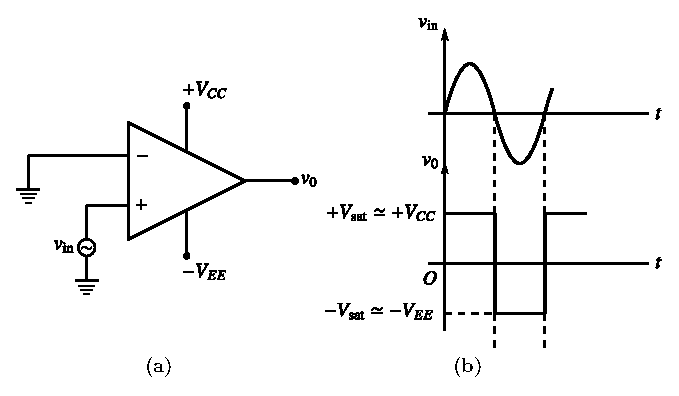
\includegraphics{chap4/fig4.4.eps}
\caption{Comparator}\label{fig4.4}
\end{figure}

Here $v_{2}=v_{\text{in}}$ and $\rmV_{1}=0$ when $v_{\text{in}}>\rmV_{1}=0$, $\rmV_{0}=+\rmV_{\text{sat}}\simeq + \rmV_{\text{CC}}$. When $\rmV_{\text{in}}<\rmV_{1}=0$, $v_{\rmo}=-\rmV_{\text{sat}}-\rmV_{\text{EE}}$. The output voltage $v_{\rmo}$ waveform is shown in Fig.~\ref{fig4.4}(b). The given circuit is known as `zero crossing detector'.

\begin{center}
\rule{4cm}{1pt}\\
{\bf\Large Problems}\\[-3pt]
\rule{4cm}{1pt}
\end{center}

\begin{problem}\label{prob4.1}
In the circuit shown in Fig.~P4.1, determine the output voltage $v_{\rmo}$. Given $A=10^{8}$.
\begin{figure}[H]
\centering
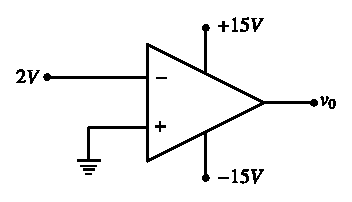
\includegraphics{chap4/figP4.1.eps}

\smallskip
{\bf Fig. P4.1}
\end{figure}
\end{problem}

\begin{solution}
Here voltage at inverting terminal is $v_{1}=2\rmV$ and non-inverting terminal is grounded i.e., $v_{2}=0\rmV$.
$$
\therefore\quad v_{\id}=v_{2}-v_{1}=0-2=-2\rmV
$$
\begin{align*}
\therefore\quad \text{Output voltage ~} v_{\rmo} &= \rmA (v_{2}-v_{1})\\[3pt]
                                             &= 10^{8}(-2)\\[3pt]
                                             &= -2\times 10^{8}\rmV.
\end{align*}
But the maximum negative voltage possible is $-\rmV_{\text{EE}}=-15\rmV$
$$
\therefore\quad v_{\rmo}=-15\rmV.
$$
\end{solution}

\noindent
{\bf Note~:} When the opamp is in open-loop configuration, the output voltage $v_{\rmo}$ is approximately +V$_{\text{CC}}$ if non-inverting terminal is at higher potential than inverting terminal and is approximately $-$V$_{\text{EE}}$ if inverting terminal is at higher potential than non-inverting terminal.

\begin{problem}\label{prob4.2}
In the circuit shown in Fig.~P4.2 draw the output voltage waveform for the input voltage waveform shown in Fig.~P4.2.1.
\begin{figure}[H]
\centering
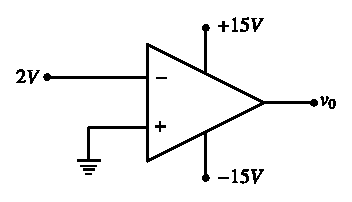
\includegraphics{chap4/figP4.1.eps}

\smallskip
{\bf Fig. P4.2}
\end{figure}
\begin{figure}[H]
\centering
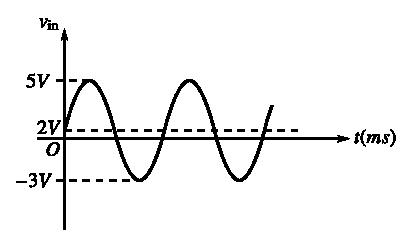
\includegraphics{chap4/figP4.2.1.eps}

\smallskip
{\bf Fig. P4.2.1}
\end{figure}
\end{problem}

\begin{solution}
Non-inverting terminal is ???????? i.e., $v_{2}=0\rmV$. When $v_{\text{in}}>0$ i.e., $v_{1}>0$, $v_{\rmo}\simeq - 15\rmV$. When $v_{\text{in}}<0$ i.e., $v_{2}<0$, $v_{\rmo}\simeq +15\rmV$. Both input and output voltage waveform are drawn in Fig.~P4.2.2.
\begin{figure}[H]
\centering
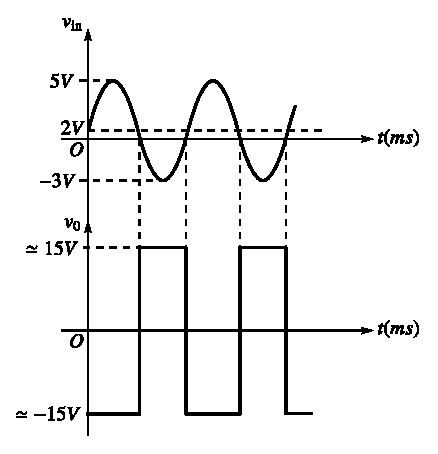
\includegraphics{chap4/figP4.2.2.eps}

\smallskip
{\bf Fig. P4.2.2}
\end{figure}
\end{solution}

\begin{problem}\label{prob4.3}
In the circuit shown in Fig.~P4.3, draw the output voltage waveform for the input voltage shown in Fig.~P4.3.1.
\begin{figure}[H]
\centering
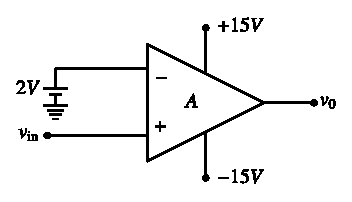
\includegraphics{chap4/figP4.3.eps}

\smallskip
{\bf Fig. P4.3}
\end{figure}
\begin{figure}[H]
\centering
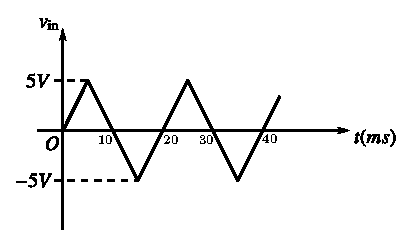
\includegraphics{chap4/figP4.3.1.eps}

\smallskip
{\bf Fig. P4.3.1}
\end{figure}
\end{problem}

\begin{solution}
The inverting terminal is $\omega t$ +2V i.e., $v_{1}=2\rmV$. When $v_{\text{in}}=\rmV_{2}>2\rmV$, $v_{\rmo}=+\rmV_{\text{sect}}=+\rmV_{\text{CC}}=+\omega \rmV$. When $v_{\text{in}}=v_{2}<2\rmV$, $v_{\rmo}=-\rmV_{\text{sat}}=-\rmV_{\text{EE}}=-15\rmV$. Output voltage $v_{\rmo}$ waveform along with input voltage waveform is shown in Fig.~P4.3.2.
\begin{figure}[H]
\centering
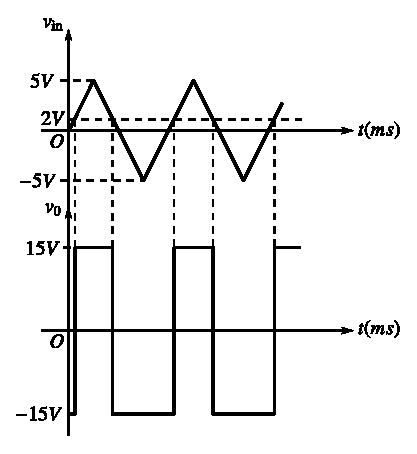
\includegraphics{chap4/figP4.3.2.eps}

\smallskip
{\bf Fig. P4.3.2}
\end{figure}
\end{solution}

\begin{problem}\label{prob4.4}
The input signal $v_{\text{in}}$ shown in Fig.~P4.4(a) is applied to the comparator circuit shown in Fig.~P4.4(b). Sketch the output voltage waveform.
\begin{figure}[H]
\centering
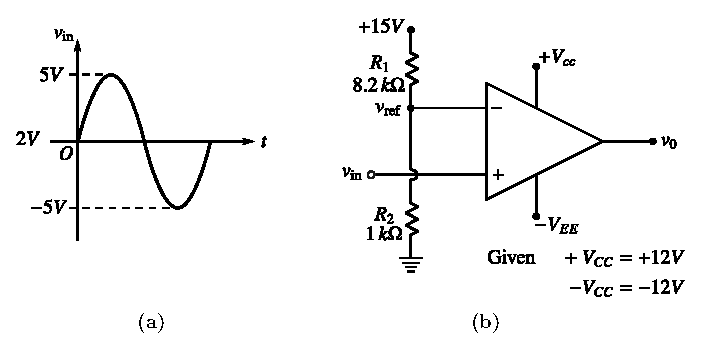
\includegraphics{chap4/figP4.4.eps}

\smallskip
{\bf Fig. P4.4}
\end{figure}
\end{problem}

\begin{solution}
Using the voltage divider rule, the voltage at the inverting terminal,
\begin{alignat*}{2}
 v_{\text{ref}} &=v_{1}=\frac{1k}{8.2 k +1k}~~ &;&\quad (+15\rmV)=1.63\rmV\\[3pt]
\therefore\quad \text{When~ } v_{\text{in}} &= v_{2}>1.63\rmV &;&\quad v_{\rmo}=+\rmV_{\text{sat}}\simeq +\rmV_{\text{CC}}\simeq + 12\rmV\\[3pt]
\text{When~ } v_{\text{in}} &=v_{2}<1.63 &;&\quad v_{\rmo}=-\rmV_{\text{sat}}\simeq -\rmV_{\text{EE}}\simeq 12\rmV
\end{alignat*}
The input and output voltage waveforms are shown in Fig.~P4.4.1 below.
\begin{figure}[H]
\centering
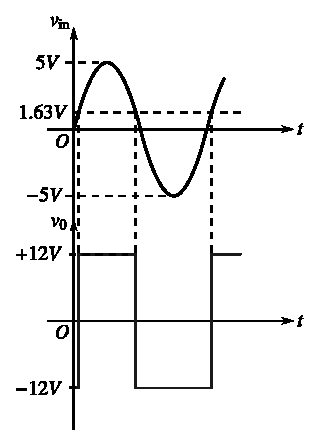
\includegraphics{chap4/figP4.4.1.eps}

\smallskip
{\bf Fig. P4.4.1}
\end{figure}
\end{solution}

\section{OPAMP Characteristics/Parameters}\label{sec4.3}

In this section, we will discuss some of the important opamp characteristics and parameters briefly.
\begin{itemize}
\item[(i)] {\it\bfseries Output offset voltage \boldmath$(\rmV_{\infty})$~:} The actual value of the output voltage, when the inputs of an opamp are zero, is called the {\em output offset voltage}. Manufacturers do not generally specify output offset voltage because it depends on the closed-loop gain that a user designs through the choice of an external component values. Instead, they specify input offset voltage and current, so that the designer can use these values to compute the output offset voltage which results in a particular application. Output offset voltage is basically due to two distinct phenomenon.

\item[(ii)] {\it\bfseries Input offset voltage} {\bf (V$_{\text{io}}$)~:} Input offset voltage is the voltage that must be applied between the two input terminals such that output voltage becomes zero.

\item[(iii)] {\it\bfseries Input bias current} {\bf (I$_{\text{B}}$)~:} It is the average of the current that flow into the inverting and non-inverting input terminals of the opamp.
\begin{equation}
\text{i.e.,~ Input bias current~~} \rmI_{\rmB}=\frac{\rmI_{\rmB 1}+\rmI_{\rmB 2}}{2}\label{eq4.2}
\end{equation}
\begin{tabbing}
where\quad \=$\rmI_{\rmB 1}$ = current into the non-inverting terminal.\\[3pt]
           \>$\rmI_{\rmB 2}$ = current into inverting terminal.
\end{tabbing}

\item[(iv)] {\it\bfseries Input offset current} {\bf (I$_{\text{io}}$)~:} It is the algebraic difference between the currents flowing into non-inverting and inverting terminals.
\begin{equation}
\text{i.e.,~ Input offset current~~} \rmI_{\text{io}}=|\rmI_{\text{B1}}-\rmI_{\text{B2}}|\label{eq4.3}
\end{equation}
\begin{tabbing}
where\quad \= $\rmI_{\text{B1}}$ = current into the non-inverting terminal.\\[3pt]
           \> $\rmI_{\text{B2}}$ = current into the inverting terminal.
\end{tabbing}

\item[(v)] {\it\bfseries Input Resistance} {\bf (R$_{\text{i}}$)~:} It is the equivalent resistance that can be measured at either the inverting or non-inverting terminal with the other terminal connected to ground.

\item[(vi)] {\it\bfseries Common Mode Rejection Ratio} {\bf (CMRR)~:} This is a figure of merit for an opamp. It is defined as the ratio of differential gain to the common mode gain.
\begin{equation}
\text{i.e.,~~ CMRR~} = \frac{\rmA_{\text{d}}}{\rmA_{\text{cm}}}\label{eq4.4}
\end{equation}
Consider the circuit shown in Fig.~\ref{fig4.4}. If the 2 input terminals of an opamp are shorted and a common signal $v_{\text{cm}}$ applied between inputs and ground, the output should be zero because $v_{\rmo}=\rmA (v_{2}-v_{1})=\rmA (v_{\text{cm}}-v_{\text{cm}})=0$.
\begin{figure}[H]
\centering
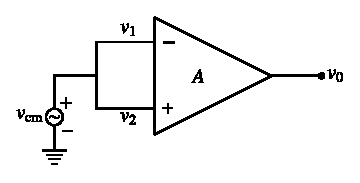
\includegraphics{chap4/fig4.5.eps}
\caption{}\label{fig4.5}
\end{figure}
However, in practical the output is non-zero and the ratio of the output voltage $v_{\rmo}$ to the input voltage $v_{\text{cm}}$ is known as {\em common mode gain} $\rmA_{\text{cm}}$. Since CMRR is very large, it is usually expressed in decibels (dB)
\begin{equation}
\text{CMRR} \Big|_{\text{dB}}= 20\log_{10}\left|\frac{\rmA_{\text{d}}}{\rmA_{\text{cm}}}\right|\label{eq4.5}
\end{equation}
Typical value of CMRR range around 100 dB. Higher the value of CMRR better the opamp.

\item[(vii)] {\it\bfseries Supply Voltage Rejection Ratio} {\bf (SVRR)~:} The change in opamp's input offset voltage $\rmV_{\text{io}}$ 'caused by variations in supply voltage is called {\em SVRR}.
\begin{equation}
\text{i.e.,~~~ SVRR} =\frac{\Delta \rmV_{\text{io}}}{\Delta \rmV}\label{eq4.6}
\end{equation}
\begin{tabbing}
\text{where\quad}~ \= $\Delta \rmV_{io}$ = change in input offset voltage\\[3pt]
                   \> $\Delta \rmV$ = change in supply voltage
\end{tabbing}

Usually, SVRR is expressed in decibels (dB)
\begin{equation}
\text{SVRR} \Big|_{\text{dB}}=20\log_{10}\left| \frac{\Delta \rmV_{\text{io}}}{\Delta \rmV}\right|\label{eq4.7}
\end{equation}
Lower the value of SVRR, better the opamp.

\item[(viii)] {\it\bfseries Slew Rate~}{\bf :} It is defined as the maximum rate of change of output voltage per unit time. It is expressed in V/$\mu$s.
\begin{equation}
\text{Slew Rate~} = \frac{\text{d}v_{\rmo}}{\text{dt}}\Big|_{\max}\label{eq4.8}
\end{equation}
Higher the slew rate, better the performance of the opamp. Slew rate indicates how fast the output of an opamp can change in response to changes in the input. The slew rate of an opamp is fixed and if the output variation with respect to time is greater than the slew rate, the distortion results.

\item[(ix)] {\it\bfseries Output Resistance} {\bf (R$_{\text{o}}$)~:} It is the equivalent resistance that can be measured between the output terminal of opamp and the ground.

\item[(x)] {\it\bfseries Gain Bandwidth product} {\bf :} It is the bandwidth of an opamp when the voltage gain is one.
\end{itemize}

\begin{center}
\rule{4cm}{1pt}\\
{\bf\Large Problems}\\[-3pt]
\rule{4cm}{1pt}
\end{center}

\begin{problem}\label{prob4.5}
Determine the input bias current and input offset current to an opamp if the current into non-inverting and inverting terminals are 8.3 $\mu$A and 7.9 $\mu$A respectively.
\end{problem}

\begin{solution}
Given $\rmI_{\text{B1}}=8.3\,\mu\rmA$, $\rmI_{\text{B2}}=7.9\,\mu \rmA$.
\begin{align*}
\text{Input bias current~ } \rmI_{\rmB} & \frac{\rmI_{\rmB 1}+\rmI_{\rmB 2}}{2}\\[2pt]
&= \frac{8.3+7.9}{2}\mu\rmA\\[2pt]
&= 8.1\mu\rmA\\[2pt]
\text{Input offset current~ } \rmI_{\text{io}} &= |\rmI_{\rmB 1}-\rmI_{\rmB 2}|\\[2pt]
&= |8.3-7.9|\mu\rmA\\[2pt]
&= 0.4 \mu\rmA
\end{align*}
\end{solution}

\begin{problem}\label{prob4.6}
A certain opamp has a differential voltage gain of 100,000 and common-mode gain of 0.25. Determine the CMRR and express it in decibels.
\end{problem}

\begin{solution}
Given~ $\rmA_{\text{d}}=100,000$, $\rmA_{\text{cm}}=0.25$.
\begin{align*}
\therefore\quad \text{CMRR~} &= \frac{\rmA_{\text{d}}}{\rmA_{\text{cm}}}=\frac{100000}{0.25}=4,00,000\\[2pt]
\text{CMRR~}\Big|_{\text{dB}} &= 20 \log_{10}(4,00,000)=112.04\text{~dB}
\end{align*}
\end{solution}

\begin{problem}\label{prob4.7}
An opamp has a differential voltage gain of 2500 and a CMRR of 30,000.
\begin{itemize}
\item[(a)] Determine the common-mode gain

\item[(b)] Express the CMRR in dB
\end{itemize}
\end{problem}

\begin{solution}
Given $\rmA_{\text{d}}=2500$, CMRR = 30,000.
\begin{itemize}
\item[(a)] We have CMRR $=\dfrac{\rmA_{\text{d}}}{\rmA_{\text{cm}}}$
$$
\therefore\quad \text{Common-mode gain~~} \rmA_{\text{cm}}=\frac{\rmA_{\text{d}}}{\text{CMRR}}=\frac{2,500}{30,000}=0.083
$$

\item[(b)] CMRR in decibels $=20\log_{10}(30,000)=89.54$ dB
\end{itemize}
\end{solution}

\vfill\eject

\begin{problem}\label{prob4.8}
When a pulse is applied to an opamp, the output voltage changes from $-8\rmV$ to +7V in 0.75 $\mu$s. What is the slew rate ?
\end{problem}

\begin{solution}
We have,
\begin{align*}
\text{slew rate~~} &= \frac{\text{d}v_{\rmo}}{\text{dt}}\Big|_{\max}\\[3pt]
&= \frac{7-(-8)}{0.75}\\[3pt]
&= 20\rmV/\mu\text{s}.
\end{align*}
\end{solution}

\begin{problem}\label{prob4.9}
How long does it take the output voltage of an opamp to go from $-10$V to $+10$V, if the slew rate is 0.5 V/$\mu$s ?
\end{problem}

\begin{solution}
We have,
\begin{align*}
\text{slew rate~~} &= \frac{\text{d}v_{\rmo}}{\dt}\\[3pt]
 \dt &= \frac{10-(-10)}{0.5}\\[3pt]
\dt &= 40 \mu \text{s}.
\end{align*}
\end{solution}

\begin{problem}\label{prob4.10}
Fig.~P4.10 below shown the output voltage $v_{\rmo}$ of an opamp in response to a step input. What is the slow rate ?
\begin{figure}[H]
\centering
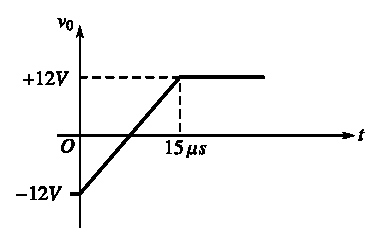
\includegraphics{chap4/fig4.11.eps}

\smallskip
{\bf Fig. P4.10}
\end{figure}
\end{problem}

\begin{solution}
We have,
\begin{align*}
\text{Slow rate~~} &= \dfrac{\text{d}v_{\rmo}}{\dt}\Big|_{\max}\\[5pt]
&= \frac{\Delta \rmV_{\rmo}}{\Delta t}=\frac{\text{Difference in output voltage}}{\text{Difference in time}}\\[5pt]
&= \frac{12-(-12)}{15\mu -0}=\frac{24}{15\mu}\\[5pt]
&= 1.6 \rmV/\mu \text{s}.
\end{align*}
\end{solution}

\begin{problem}\label{prob4.11}
An opamp has a common input signal of 3.20V to both the terminals. This results in an output signal of 26 mV. Determine the common mode gain and the CMRR. Given that the differential gain is 100.
\end{problem}

\begin{solution}
Common-mode gain $\rmA_{\text{cm}}=\dfrac{v_{\rmo}}{v_{\text{cm}}}=\dfrac{26\times 10^{-3}}{3.2}=0.0081$
\begin{align*}
&\therefore\quad \text{CMRR~} = \frac{\rmA_{\text{d}}}{\rmA_{\text{cm}}}=\frac{100}{0.0081}=12345.6\\[4pt]
&\therefore\quad \text{CMRR~}\big|_{\text{dB}}=20\log_{10}(12345.6)=81.8\;\text{dB}
\end{align*}
\end{solution}

\section{Ideal Opamp}\label{sec4.4}

An ideal opamp exhibits the following electrical properties.
\begin{itemize}
\item[(i)] Infinite voltage gain

\item[(ii)] Infinite input resistance

\item[(iii)] Zero output resistance

\item[(iv)] Zero input offset voltage

\item[(v)] Zero input offset current

\item[(vi)] Infinite bandwidth

\item[(vii)] Infinite CMRR

\item[(viii)] Infinite slew rate

\item[(ix)] Zero SVRR

\item[(x)] The characteristics of an opamp do not change with temperature
\end{itemize}

\section{Need for Opamp}\label{sec4.5}

Consider the case of adding two signals $v_{1}$ and $v_{2}$ using resistors $\rmR_{1}$ and $\rmR_{2}$ as shown and $\rmR_{\rmL}$ is the load resistor.
\begin{figure}[H]
\centering
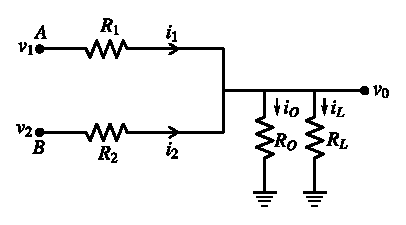
\includegraphics{chap4/fig4.6.eps}
\caption{Summing two voltages}\label{fig4.6}
\end{figure}

Applying KCL at junction,
\begin{align}
& \rmi +\rmi=\rmi_{0}+\rmi_{\rmL}\label{eq4.9}\\[3pt]
& \frac{v_{1}-v_{\rmo}}{\rmR_{1}}+\frac{v_{2}-v_{\rmo}}{\rmR_{2}}=\frac{v_{\rmo}}{\rmR_{\rmo}}+\frac{v_{\rmo}}{\rmR_{\rmL}}\notag\\[3pt]
& v_{\rmo}\left[\frac{1}{\rmR_{\rmo}}+\frac{1}{\rmR_{L}}+\frac{1}{\rmR_{1}}+\frac{1}{\rmR_{2}}\right]=\frac{v_{1}}{\rmR_{1}}+\frac{v_{2}}{\rmR_{2}}\label{eq4.10}
\end{align}

Consider $\rmR_{\rmP}$ is a parallel combination of $\rmR_{\rmo}$ and $\rmR_{L}$
\begin{equation}
\text{i.e.,}\quad \frac{1}{\rmR_{\rmP}}=\frac{1}{\rmR_{\rmo}}+\frac{1}{\rmR_{L}}\label{eq4.11}
\end{equation}

Substituting Eqn.~\eqref{eq4.11} in Eqn.~\eqref{eq4.10},
$$
v_{\rmo}\left[\frac{1}{\rmR_{\rmP}}+\frac{1}{\rmR_{1}}+\frac{1}{\rmR_{2}}\right]=\frac{v_{1}}{\rmR_{1}}+\frac{v_{2}}{R_{2}}
$$

$\therefore$~ The output voltage
\begin{equation}
v_{\rmo}=\frac{(v_{1}/\rmR_{1})+(v_{2}/\rmR_{2})}{\left[\frac{1}{R_{\rmP}}+\frac{1}{\rmR_{1}}+\frac{1}{\rmR_{2}}\right]}\label{eq4.12}
\end{equation}

Multiplying both numerator and denominator by $\rmR_{\rmP}$, we get,
\begin{equation}
v_{\rmo}=\frac{v_{1}(\rmR_{\rmP}/\rmR_{1})+v_{2}(\rmR_{\rmP}/\rmR_{2})}{\left[1+\frac{\rmR_{\rmP}}{\rmR_{1}}+\frac{\rmR_{P}}{\rmR_{2}}\right]}\label{eq4.13}
\end{equation}

From Eqn.~\eqref{eq4.13}, it is clear that the output voltage $v_{\rmo}$ depends on $\rmR_{\rmL}$. If it is required to make $v_{\rmo}$ independent of $\rmR_{\rmL}$, it is then necessary to choose $\rmR_{\rmo}\ll \rmR_{\rmL}$. But this results in a large signal attenuation which is undesirable.

To overcome this problem of large signal attenuation, an amplifier with some gain must be used. But the use of conventional amplifier such as RC coupled amplifier will not amplify dc voltages because of coupling capacitances. With transformer coupling dc signals cannot be amplified. Direct coupled amplifier may not be employed because the gain of a single stage in direct coupling is limited, so many stages have to be used. Moreover, the design of such a complicated circuit requires advance knowledge of circuit design.

Therefore, the best way to overcome these problems is to use opamp because the closed-loop gain of an opamp depends only on circuit components external to it and is independent of its open-loop gain. Thus the opamp is a well suited electronic device whose use overcomes all the above unwanted problems which are present if a conventional amplifier is used.

\section{Opamp Applications}\label{sec4.6}

Using opamp in closed loop configuration i.e., by connecting a component from output to input externally, opamp may be used for different applications. Very few of them are mentioned below.
\begin{itemize}
\itemsep=0pt
\item[(i)] Inverting amplifier

\item[(ii)] Non-inverting amplifier

\item[(iii)] Voltage follower

\item[(iv)] Adder and Subtractor

\item[(v)] Differentiator

\item[(vi)] Integrator
\end{itemize}

\noindent
{\bf Note~:} We have
\begin{equation}
v_{\rmo}=\rmA \, v_{\id}=\rmA(v_{2}-v_{1})\label{eq4.14}
\end{equation}
\begin{tabbing}
where\quad \= A = open-loop gain of opamp.\\[3pt] 
           \> $v_{\id}$ = difference input voltage (V)\\[3pt]
           \> $v_{2}$ = voltage at non-inverting terminal with respect to ground (V)\\[3pt]
           \> $v_{1}$ = voltage at inverting terminal with respect to ground (V)\\[3pt]
           \> $v_{\rmo}$ = output voltage (V) 
\end{tabbing}

From Eqn.~\eqref{eq4.14}, we have
\begin{equation}
\rmA =\frac{v_{\rmo}}{v_{\id}}=\frac{v_{\rmo}}{v_{2}-v_{1}}\label{eq4.15}
\end{equation}

Ideally, open-loop gain is infinity.
\begin{align}
&\therefore\quad v_{2}-v_{1}\simeq 0\notag\\
&\therefore\quad v_{1}\simeq v_{2}\label{eq4.16}
\end{align}

\subsection{Inverting Amplifier}\label{sec4.6.1}

An opamp connected as an inverting amplifier is shown in Fig.~\ref{fig4.7}. The input signal $v_{\text{in}}$ is applied through a series input resistor $\rmR_{1}$ to the inverting input. Also, the output is fed back through $\rmR_{\rmf}$ to the same input. The non-inverting terminal is grounded.
\begin{figure}[H]
\centering
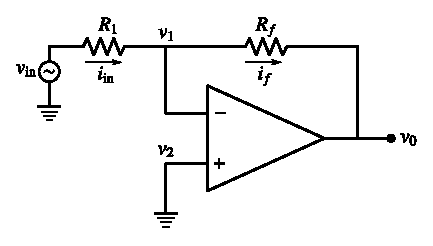
\includegraphics{chap4/fig4.7.eps}
\caption{Inverting Amplifier}\label{fig4.7}
\end{figure}

We know that the input resistance $\rmR_{\rmi}$ of an opamp is very large (ideally infinity). Therefore, there is no current at the inverting input. So the current through $\rmR_{1}$ and $\rmR_{\rmf}$ must be equal.
\begin{align}
\text{i.e.,}\quad \rmi_{\text{in}} &= \rmi_{\rmf}\label{eq4.17}\\[3pt]
\frac{v_{\text{in}}-v_{1}}{\rmR_{1}} &= \frac{v_{1}-v_{\rmo}}{\rmR_{f}}\label{eq4.18}
\end{align}

Since non-inverting terminal is grounded, $v_{1}=0$.

$\therefore$~ From Eqn.~\eqref{eq4.16}, $v_{1}\simeq v_{2}$.

$\therefore$~ From Eqn.~\eqref{eq4.18},
\begin{align}
\frac{v_{\text{in}}}{\rmR_{1}} &= -\frac{v_{\rmo}}{\rmR_{\rmf}}\notag\\[3pt]
\therefore\quad v_{\rmo} &= -\frac{\rmR_{\rmf}}{\rmR_{1}}\cdot v_{\text{in}}\notag\\[3pt]
\therefore\quad \text{Closed loop gain~~ } \rmA_{\rmf} &= \frac{v_{\rmo}}{v_{\text{in}}}=-\frac{\rmR_{\rmf}}{\rmR_{1}}\label{eq4.19}
\end{align}

Eqn.~\eqref{eq4.19} shows that the closed-loop gain $\rmA_{\rmf}$ of an inverting amplifier is the ratio of the feedback resistance $\rmR_{\rmf}$ to the resistance $\rmR_{1}$. The closed-loop gain is independent of internal open-loop gain of the opamp. The negative sign in Eqn.~\eqref{eq4.19} indicates that there is a phase inversion between output and input voltage.

The impedance seen from the source $v_{\text{in}}$ is,
\begin{equation}
\rmR_{\text{in}}=\frac{v_{\text{in}}}{\rmi_{\text{in}}}=\rmR_{1}\label{eq4.20}
\end{equation}

\begin{center}
\rule{4cm}{1pt}\\
{\bf\Large Problems}\\[-3pt]
\rule{4cm}{1pt}
\end{center}

\begin{problem}\label{prob4.12}
Given the opamp circuit shown in Fig.~P4.12, determine the value of $\rmR_{\rmf}$ required to obtain a closed-loop voltage gain of $-50$.
\begin{figure}[H]
\centering
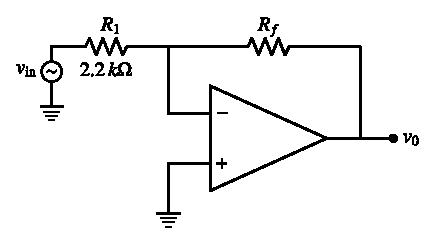
\includegraphics{chap4/figP4.12.eps}

\smallskip
{\bf Fig. P4.12}
\end{figure}
\end{problem}

\begin{solution}
The given circuit is an inverting amplifier.

$\therefore$~ The closed-loop voltage gain $\rmA_{\rmf}=-\dfrac{\rmR_{\rmf}}{\rmR_{1}}$

Given
\begin{align*}
\rmA_{\rmf}=-50, ~ \rmR_{1} &= 2.2~ \rmk\Omega\\[3pt]
\therefore\quad \rmR_{\rmf} &= -\rmA_{\rmf}\rmR_{1}\\[3pt]
&= -(-50)\times 2.2\times 10^{3}\\[3pt]
\rmR_{\rmf} &= 100~ \rmk \Omega
\end{align*}
\end{solution}

\begin{problem}\label{prob4.13}
For the inverting amplifier shown in Fig.~P4.13, calculate the values of $\rmA_{\rmf}$ and $\rmR_{\text{in}}$.
\begin{figure}[H]
\centering
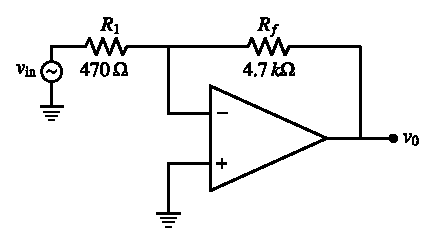
\includegraphics{chap4/figP4.13.eps}

\smallskip
{\bf Fig. P4.13}
\end{figure}
\end{problem}

\begin{solution}
Given $\rmR_{1}=470\,\Omega$, $\rmR_{\rmf}=4.7\,\rmk\Omega$
\begin{align*}
\therefore\quad \text{Closed-loop gain~~ } \rmA_{\text{f}} &= -\frac{\rmR_{\rmf}}{\rmR_{1}}=\frac{4.7\times 10^{3}}{470}\\[3pt]
\therefore\quad \rmA_{\rmf} &= -10
\end{align*}

Resistance seen from the source $\rmR_{\text{in}}=\rmR_{1}=470\,\Omega$.
\end{solution}

\begin{problem}\label{prob4.14}
For the circuit of inverting amplifier $\rmR_{\rmf}=100 \rmk\Omega$, $\rmR_{1}=10 \rmk\Omega$ and $v_{\text{in}}=1\rmV$, calculate
\begin{itemize}
\item[(i)] Closed-loop gain $\rmA_{\rmf}$

\item[(ii)] Output voltage $v_{\rmo}$

\item[(iii)] Input current $\rmi_{\text{in}}$

\item[(iv)] Feedback current $\rmi_{\rmf}$
\end{itemize}
\end{problem}

\begin{solution}
Given $\rmR_{\rmf}=100 \rmk\Omega$, $\rmR_{1}=10 \rmk \Omega$, $v_{\text{in}}=1\rmV$.
\begin{itemize}
\item[(i)] Closed-loop gain $\rmA_{\rmf}=-\frac{\rmR_{\rmf}}{\rmR_{1}}=-\frac{100\times 10^{3}}{10\times 10^{3}}=-10$

\item[(ii)] Output voltage $v_{\rmo}=\rmA_{\rmf}v_{\text{in}}=(-10)(1)=-10\rmV$

\item[(iii)] Input current
\begin{align*}
\rmi_{\text{in}} &= \frac{v_{\text{in}}-v_{1}}{\rmR_{1}}\\[3pt]
\rmi_{\text{in}} &= \frac{v_{\text{in}}}{\rmR_{1}}\quad [\because \ v_{1}\simeq v_{2}\simeq 0]\\[3pt]
\rmi_{\text{in}} &= \frac{1}{10\times 10^{3}}=0.1\text{~mA}
\end{align*}

\item[(iv)] Feedback current $\rmi_{\rmf}=\rmi_{\text{in}}=0.1$~mA
\end{itemize}
We have $v_{1}=v_{2}$. Since $v_{2}=0$, $v_{1}$ is also at ground potential i.e., $v_{1}=0$. This concept is called `virtual ground.
\end{solution}

\begin{problem}\label{prob4.15}
Determine the closed-loop gain and input resistance seen by source in the circuit shown in Fig.~P4.15.
\begin{figure}[H]
\centering
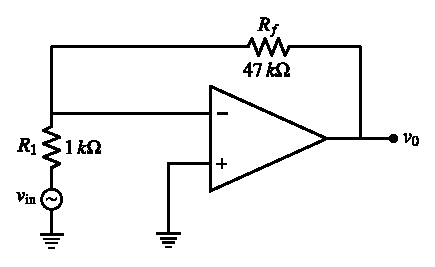
\includegraphics{chap4/figP4.15.eps}

\smallskip
{\bf Fig. P4.15}
\end{figure}
\end{problem}

\begin{solution}
The given circuit in Fig.~P4.15 is an inverting amplifier with $\rmR_{1}=1\,\rmk\Omega$ and $\rmR_{\rmf}=47\, \rmk\Omega$.

$\therefore$\quad Closed-loop gain $\rmA_{\rmf}=-\dfrac{\rmR_{\rmf}}{\rmR_{1}}=-\dfrac{47\times 10^{3}}{1\times 10^{3}}=-47$

\medskip
Input resistance $\rmR_{\text{in}}=\rmR_{1}=1\,\rmk\Omega$
\end{solution}

\begin{problem}\label{prob4.16}
If a signal voltage of 10 mV$_{\text{rms}}$ is applied to the inverting amplifier shown in Fig.~P4.16, what is the output voltage and what is its phase relationship with the input ?
\begin{figure}[H]
\centering
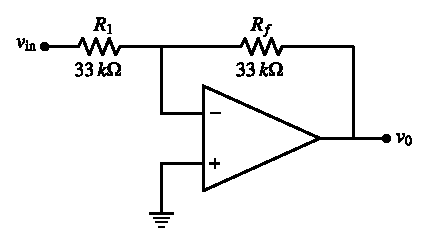
\includegraphics{chap4/figP4.16.eps}

\smallskip
{\bf Fig. P4.16}
\end{figure}
\end{problem}

\begin{solution}
Given $v_{\text{in}}=10$ mV$_{\text{rms}}$, $R_{1}=33$ k$\Omega$, $\rmR_{\rmf}=33$\,k$\Omega$.
\begin{align*}
\rmA_{\rmf} = \frac{v_{\rmo}}{v_{\text{in}}} &= -\frac{\rmR_{\rmf}}{\rmR_{1}}\\[3pt]
\therefore\quad v_{\rmo} &= -\frac{R_{\rmf}}{\rmR_{1}}\cdot v_{\text{in}}\\[3pt]
&= -\frac{33\times 10^{3}}{33\times 10^{3}}\times 10\times 10^{-3}
\end{align*}
$\therefore$~ Output voltage $=v_{\rmo}=-10$\,mV.

\smallskip
The output voltage $v_{\rmo}$ is out of phase with input voltage $v_{\text{in}}$.
\end{solution}

\begin{problem}\label{prob4.17}
For the inverting amplifier shown in Fig.~P4.17, determine $\rmA_{\rmf}$, $v_{\rmo}$, $\rmi_{\text{in}}$, $\rmi_{\rmf}$, $\rmi_{\rmL}$ and $\rmi_{\rmO}$.
\begin{figure}[H]
\centering
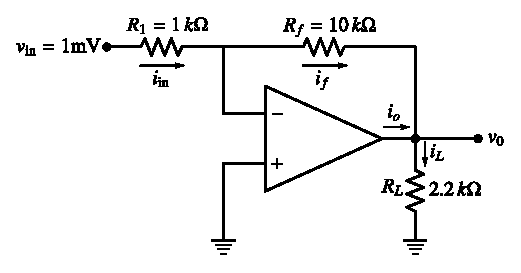
\includegraphics{chap4/figP4.17.eps}

\smallskip
{\bf Fig. P4.17}
\end{figure}
\end{problem}

\begin{solution}
Given $v_{\text{in}}=1$ mV, $\rmR_{1}=1$ k$\Omega$, $\rmR_{\rmf}=10$ k$\Omega$

\medskip
Closed-loop gain $\rmA_{\rmf}=-\dfrac{\rmR_{\rmf}}{\rmR_{1}}=-\dfrac{10\times 10^{3}}{1\times 10^{3}}=-10$

\medskip
Output voltage $v_{\rmo}=\rmA_{f}v_{\text{in}}=(-10)(1\times 10^{-3})=-10$ mV

\medskip
Input current $\rmi_{\text{in}}=\dfrac{v_{\text{in}}}{\rmR_{1}}=\dfrac{1\times 10^{-3}}{1\times 10^{3}}=1\mu\rmA$

\medskip
Feedback current $\rmi_{\rmf}=\rmi_{\text{in}}=1\,\mu$A

\medskip
Load current $\rmi_{L}=\dfrac{v_{\rmo}}{\rmR_{\rmL}}=-\dfrac{10\times 10^{-3}}{2.2\times 10^{3}}=-4.55\mu\rmA$

\eject

Total output current
\begin{align*}
\rmi_{0} &= \rmi_{\rmf}+\rmi_{\rmL}\\[3pt]
&= (1-4.55)\mu\rmA\\[3pt]
\rmi_{0} &= -3.55\mu\rmA
\end{align*}
\end{solution}

\subsection{Non-inverting Amplifier}\label{sec4.6.2}

An opamp connected as a non-inverting amplifier, is shown in Fig.~\ref{fig4.8}. The input signal $v_{\text{in}}$ is applied to the non-inverting input. The output is applied back to the inverting input through the feedback circuit formed by resistors $\rmR_{1}$ and $\rmR_{\rmf}$.
\begin{figure}[H]
\centering
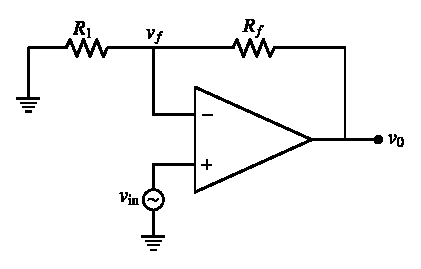
\includegraphics{chap4/fig4.8.eps}
\caption{Non-inverting amplifier}\label{fig4.8}
\end{figure}


The closed-loop gain
\begin{equation}
\rmA_{\rmf}=\frac{v_{\rmo}}{v_{\text{in}}}\label{eq4.21}
\end{equation}

Also we have
\begin{equation}
v_{\rmo}=\rmA (v_{2}-v_{1})\label{eq4.22}
\end{equation}

From Fig.~\ref{fig4.8}, we have $v_{2}=v_{\text{in}}$\hfill (4.23)

$\rmR_{\rmf}$ and $\rmR_{1}$ form a voltage divider.
\setcounter{equation}{23}
\begin{equation}
\therefore\quad v_{1}=v_{\rmf}=\dfrac{\rmR_{1}}{\rmR_{1}+\rmR_{\rmf}}\cdot v_{\rmo}\label{eq4.24}
\end{equation}

Substituting Eqn.~(4.23) and \eqref{eq4.24} in Eqn.~\eqref{eq4.22}, we get
\begin{equation}
v_{\rmo}=A\left(v_{\text{in}}-\dfrac{\rmR_{1}v_{\rmo}}{\rmR_{1}+\rmR_{\rmf}}\right)\label{eq4.25}
\end{equation}

Re-arranging Eqn.~\eqref{eq4.25}, we get
\begin{equation}
v_{\rmo}=\dfrac{\rmA (\rmR_{1}+\rmR_{\rmf})v_{\text{in}}}{\rmR_{1}+\rmR_{\rmf}+\rmA\rmR_{1}}\label{eq4.26}
\end{equation}

The open-loop gain $\rmA$ of an opamp is very large (ideally infinity).
$$
\text{So,}\quad \rmA\rmR_{1}\gg (\rmR_{1}+\rmR_{\rmf})\quad\therefore\quad \rmR_{1}+\rmR_{\rmf}+\rmA\rmR_{1}\simeq \rmA\rmR_{1}.
$$

$\therefore$~ Eqn.~\eqref{eq4.26} reduces to,
\begin{gather}
v_{\rmo}\simeq \dfrac{\rmA(\rmR_{1}+\rmR_{\rmf})}{\rmA\rmR_{1}}\cdot v_{\text{in}}\notag\\
\therefore\quad \text{Closed-loop gain~~ } \rmA_{\rmf}=\frac{v_{\rmo}}{v_{\text{in}}}=1+\frac{\rmR_{\rmf}}{\rmR_{1}}\label{eq4.27}
\end{gather}

Notice that the closed-loop voltage gain is not at all dependent on the open-loop voltage gain of opamp. The value of closed-loop voltage gain $\rmA_{\rmf}$ can be set by selecting values of external resistors $\rmR_{1}$ and $\rmR_{\rmf}$.

\begin{center}
\rule{4cm}{1pt}\\
{\bf\Large Problems}\\[-3pt]
\rule{4cm}{1pt}
\end{center}

\begin{problem}\label{prob4.18}
Determine the gain of the amplifier shown in Fig.~P4.18.
\begin{figure}[H]
\centering
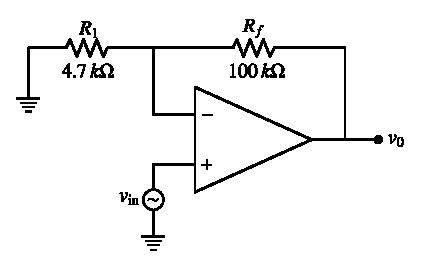
\includegraphics{chap4/figP4.18.eps}

\smallskip
{\bf Fig. P4.18}
\end{figure}
\end{problem}

\begin{solution}
The circuit given is a non-inverting amplifier with $\rmR_{1}=4.7$ k$\Omega$ and $\rmR_{\rmf}=100$ k$\Omega$.

$\therefore$~ The closed-loop gain
\begin{align*}
\rmA_{\rmf} &= 1+\frac{\rmR_{\rmf}}{\rmR_{1}}\\[3pt]
          &= 1+\frac{100\times 10^{3}}{4.7\times 10^{3}}\\[3pt]
\rmA_{\rmf} &= 22.3.
\end{align*}
\end{solution}

\begin{problem}\label{prob4.19}
For the circuit of non-inverting amplifier shown in Fig.~P4.19, determine
\begin{itemize}
\item[(i)] closed-loop gain $\rmA_{\rmf}$

\item[(ii)] output voltage $v_{\rmo}$
\end{itemize}
\begin{figure}[H]
\centering
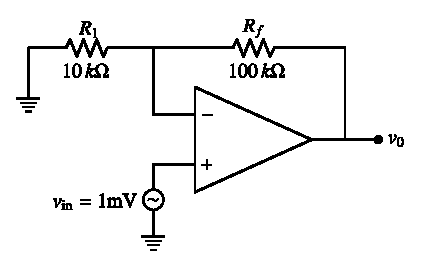
\includegraphics{chap4/figP4.19.eps}

\smallskip
{\bf Fig. P4.19}
\end{figure}
\end{problem}

\begin{solution}
Given $v_{\text{in}}=1$ mV, $\rmR_{1}=10\,\rmk \Omega$, $\rmR_{\rmf}=100\,\rmk\Omega$
\begin{itemize}
\item[(i)] 
\begin{tabbing}
Closed-loop gain~~ $\rmA_{\rmf}$ \== $1+\dfrac{\rmR_{\rmf}}{\rmR_{1}}$\\[4pt]
                                \>= $1+\dfrac{100\times 10^{3}}{10\times 10^{3}}$\\[4pt]
\phantom{aaaaaaaaaaqqqqqq,}$\rmA_{\rmf}$ \>= 11.
\end{tabbing}

\item[(ii)] Output voltage~ $v_{\rmo}=\rmA_{\rmf}$, $v_{\text{in}}=11\times 1\times 10^{-3}=11$ mV.
\end{itemize}
\end{solution}

\begin{problem}\label{prob4.20}
Determine the closed-loop gain of the amplifier shown in Fig.~P4.20.
\begin{figure}[H]
\centering
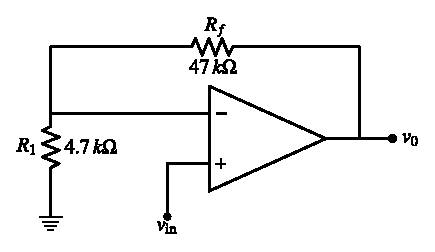
\includegraphics{chap4/figP4.20.eps}

\smallskip
{\bf Fig. P4.20}
\end{figure}
\end{problem}

\begin{solution}
The circuit given in Fig.~P4.20 is a non-inverting amplifier with $\rmR_{1}=4.7$ k$\Omega$ and $\rmR_{\rmf}=47$ k$\Omega$.

$\therefore$~ Closed-loop gain
\begin{align*}
\rmA_{\rmf} &= 1+\frac{\rmR_{\rmf}}{\rmR_{1}}= 1+\frac{47\times 10^{3}}{4.7\times 10^{3}}\\[3pt]
\rmA_{\rmf} &= 11
\end{align*}
\end{solution}

\begin{problem}\label{prob4.21}
Find the value of $\rmR_{\rmf}$ that will produce a closed-loop gain of 8 in the non-inverting amplifier shown in Fig.~P4.21.
\begin{figure}[H]
\centering
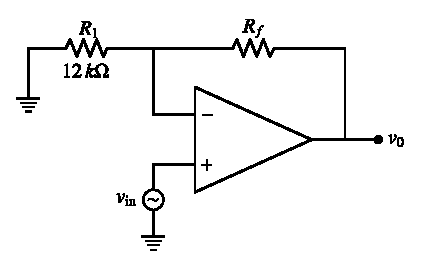
\includegraphics[scale=.95]{chap4/figP4.21.eps}

\smallskip
{\bf Fig. P4.21}
\end{figure}
\end{problem}

\begin{solution}
Given $\rmR_{1}=12$ k$\Omega$, $\rmA_{\rmf}=8$

\medskip
We have $\rmA_{\rmf}=1+\dfrac{\rmR_{\rmf}}{\rmR_{1}}$
\begin{align*}
\therefore\quad \rmR_{\rmf} &= \rmR_{1}(\rmA_{f}-1)= 12\times 10^{3}\times (8-1)\\[3pt]
\therefore\quad \rmR_{\rmf} &= 844 \rmk \Omega
\end{align*}
\end{solution}

\begin{problem}\label{prob4.22}
For the cascaded amplifier shown in Fig.~P4.22, determine the output voltage $v_{\rmo}$.
\begin{figure}[H]
\centering
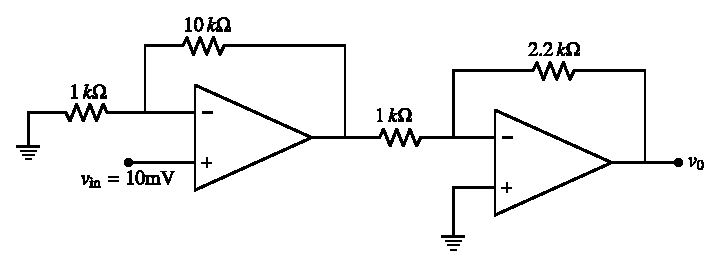
\includegraphics[scale=.95]{chap4/figP4.22.eps}

\smallskip
{\bf Fig. P4.22}
\end{figure}
\end{problem}

\vfill\eject

\begin{solution}
In the circuit shown in Fig.~P4.22, the first stage is a non-inverting amplifier and second stage is an inverting amplifier.

\medskip
Gain of first stage\quad $\rmA_{\rmf 1}=1+\dfrac{\rmR_{\rmf}}{\rmR_{1}}=1+\dfrac{10\times 10^{3}}{1\times 10^{3}}=11$

\medskip
Gain of second stage\quad $\rmA_{\rmf 2}=-\dfrac{\rmR_{\rmf}}{\rmR_{1}}=\dfrac{2.2\times 10^{3}}{1\times 10^{3}}=-2.2$

\medskip
$\therefore$~ Overall voltage gain $\rmA_{\rmf}=\rmA_{\rmf 1}\cdot \rmA_{\rmf 2}=11(-2.2)=-24.2$

\medskip
\begin{tabbing}
\quad~~$\therefore$~ Output voltage $v_{\rmo}=\rmA_{\rmf}~v_{\text{in}}$ \== $(-24.2)(10\times 10^{-3})$\\[4pt]
\phantom{AAiAAAAAAAAAAAAA} $\therefore$~ $v_{\rmo}$ \>= $-242$ mV
\end{tabbing}
\end{solution}

\subsection{Voltage follower}\label{sec4.6.3}

The voltage follower is a special case of non-inverting amplifier, where all the output voltage is fed back to the inverting input by a straight connection as shown in Fig.~\ref{fig4.9}.
\begin{figure}[H]
\centering
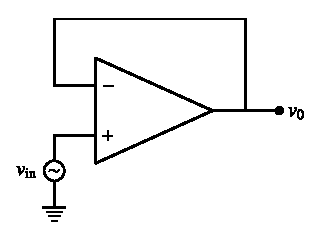
\includegraphics{chap4/fig4.19.eps}
\caption{Voltage Follower}\label{fig4.9}
\end{figure}

Comparing this circuit with non-inverting amplifier shown in Fig.~\ref{fig4.8}, we notice that $\rmR_{\rmf}=0$ and $\rmR_{1}=\infty$. Therefore, the closed-loop voltage gain.
\begin{align}
\rmA_{\rmf} &= 1+\frac{\rmR_{\rmf}}{\rmR_{1}}=1+\frac{0}{\infty}=1\notag\\[3pt]
\text{i.e.,}\quad \rmA_{\rmf} &=1\label{eq4.28}\\[3pt]
\therefore\quad v_{\rmo} &= v_{\text{in}}\notag
\end{align}

Since the output voltage $v_{0}$ has the same magnitude and phase as $v_{\text{in}}$, this configuration is called a {\em voltage follower}. This circuit is used in applications where, power gain and impedence isolation are of primary concern.

\begin{problem}\label{prob4.23}
If a input signal voltage of 10 mV is applied to each amplifier in Fig.~P4.23(a), (b), (c) and (d) shown below, what are the output voltages and what is their phase relationship with inputs.
\begin{figure}[H]
\centering
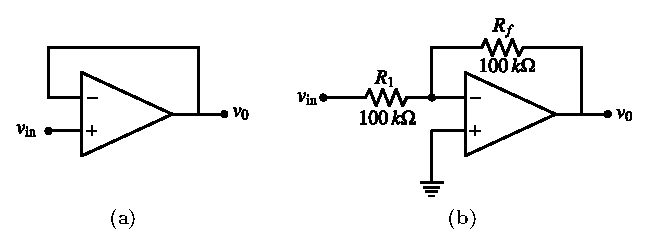
\includegraphics{chap4/figP4.23ab.eps}

\bigskip
\smallskip

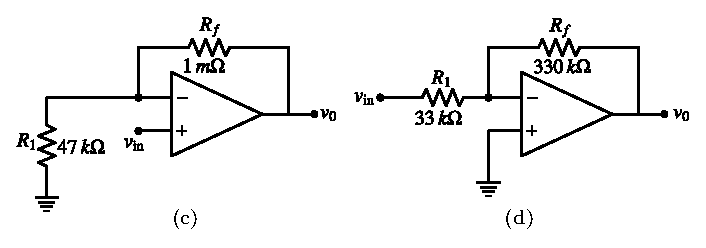
\includegraphics{chap4/figP4.23cd.eps}

\medskip
{\bf Fig. P4.23}
\end{figure}
\end{problem}

\begin{solution}
Given $v_{\text{in}}=10$ mV
\begin{itemize}
\item[(a)] It is a voltage follower.
\begin{align*}
\therefore\quad & \rmA_{v}=\frac{v_{\rmo}}{v_{\text{in}}}=1\\[5pt]
\therefore\quad & v_{\rmo}=v_{\text{in}}=10\text{~mV}
\end{align*}

\item[(b)] It is an inverting amplifier.
\begin{align*}
& \rmA_{v} \frac{\rmA_{\rmo}}{\rmV_{\text{in}}}=-\frac{\rmR_{\rmf}}{\rmR_{1}}=-\frac{100\text{~k}}{100\text{~k}}=-1\\[5pt]
& v_{\rmo}=-v_{\text{in}}=-10\text{~mV.}
\end{align*}
$v_{\rmo}$ is out of phase with $v_{\text{in}}$.

\eject

\item[(c)] It is a non-inverting amplifier.
\begin{align*}
\rmA_{v} &= \frac{v_{\rmo}}{v_{\text{in}}}=1+\frac{\rmR_{\rmf}}{\rmR_{1}}=1+\frac{1\rmm}{47\rmk}=22.28\\[4pt]
\therefore\quad v_{\rmo} &= 22.28 v_{\text{in}}=22.28\times 10\times 10^{-3}=222.77\text{~mV}
\end{align*}
$v_{\rmo}$ is in-phase with $v_{\text{in}}$.

\item[(d)] It is an inverting amplifier.
\begin{align*}
\rmA_{v} &= \frac{v_{\rmo}}{v_{\text{in}}}=-\frac{\rmR_{\rmf}}{\rmR_{1}}=-\frac{330\rmk}{33\rmk}=-10\\[4pt]
\therefore\quad v_{\rmo} &=-10v_{\text{in}}=-10\times 10\times 10^{-3}=-100\text{~mV}
\end{align*}
$v_{\rmo}$ is out of phase with $v_{\text{in}}$.
\end{itemize}
\end{solution}

\begin{problem}\label{prob4.24}
Find the value of $\rmR_{\rmf}$ that will produce the indicated closed loop gain in each amplifier in Fig.~P4.24(a), (b) and (c) shown below.
\begin{figure}[H]
\centering
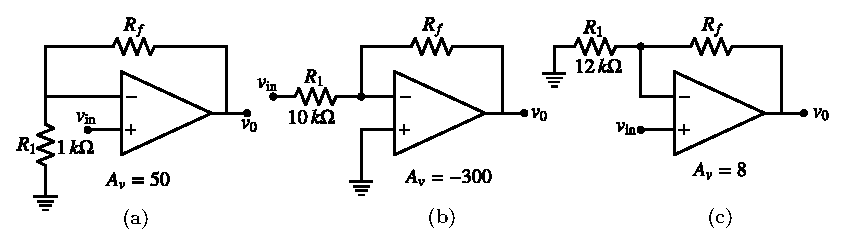
\includegraphics{chap4/figP4.24.eps}

\smallskip
{\bf Fig. P4.24}
\end{figure}
\end{problem}

\begin{solution}
\begin{itemize}
\item[(a)] It is non-inverting amplifier.

Given\quad $\rmA_{v}=50$ and $\rmR_{1}=1$~k$\Omega$

We have
\begin{align*}
\rmA_{v} &= 1+\frac{\rmR_{\rmf}}{\rmR_{1}}=50\\[4pt]
\therefore\quad \rmR_{\rmf} &= 49\text{~k}\Omega
\end{align*}

\eject

\item[(b)] It is an inverting amplifier.

Given\quad $\rmR_{v}=-300$ and $\rmR_{1}=10$~k$\Omega$.

We have
\begin{align*}
\rmA_{v} &= -\frac{\rmR_{\rmf}}{\rmR_{1}}=-300\\[3pt]
\therefore\quad \rmR_{\rmf} &= 3\text{~M}\Omega
\end{align*}

\item[(c)] It is non-inverting amplifier.

Given\quad $\rmA_{v}=8$ and $\rmR_{1}=12$~k$\Omega$

We have
\begin{align*}
\rmA_{v} &= 1+\frac{\rmR_{\rmf}}{\rmR_{1}}=8\\[3pt]
\therefore\quad \rmR_{\rmf} &= 84\text{~k}\Omega
\end{align*}
\end{itemize}
\end{solution}

\subsection{Adder and Subtractor}

The circuit which provides an output voltage proportional or equal to algebraic sum of two or more input voltages, multiplied by a constant gain factor is called an adder or summer.

\smallskip
\itheading{Adder in inverting configuration}~: Consider an opamp in inverting configuration as shown in Fig.~\ref{fig4.10}. Three resistors $\rmR_{\rma}$, $\rmR_{\rmb}$ and $\rmR_{\rmc}$ are connected to the inverting terminal. Signals $\rmV_{\rma}$, $\rmV_{\rmb}$ and $\rmV_{\rmc}$ are fed to the opamp through $\rmR_{\rma}$, $\rmR_{\rmb}$ and $\rmR_{\rmc}$ respectively.
\begin{figure}[H]
\centering
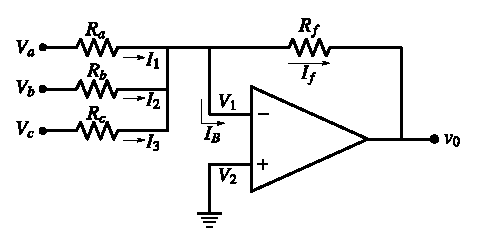
\includegraphics{chap4/fig4.10.eps}
\caption{A summer using opamp}\label{fig4.10}
\end{figure}

Applying KCL at node $v_{1}$, 
\begin{equation}
\rmI_{1}+\rmI_{2}+\rmI_{3}=\rmI_{a}+\rmI_{f}\label{eq4.29}
\end{equation}

Since input resistance $\rmR_{\rmi}$ of an opamp is very large $\rmI_{\rmB}\simeq 0$. Therefore from Eqn.~\eqref{eq4.29}.
\begin{align}
\rmI_{1}+\rmI_{2}+\rmI_{3} &\simeq \rmI_{\rmf}\notag\\[3pt]
\frac{\rmV_{\rma}-\rmV_{2}}{\rmR_{\rma}}+\frac{\rmV_{\rmb}-\rmV_{2}}{\rmR_{\rmb}} &+ \frac{\rmV_{\rmc}-\rmV_{2}}{\rmR_{\rmc}}=\frac{\rmV_{2}-\rmV_{0}}{\rmR_{\rmF}}\label{eq4.30}
\end{align}

Since $v_{1}=v_{2}=0$, we have
\begin{align}
& \frac{\rmV_{\rma}}{\rmR_{\rma}}+\frac{\rmV_{\rmb}}{\rmR_{\rmb}}+\frac{\rmV_{\rmc}}{\rmR_{\rmc}}=-\frac{\rmV_{0}}{\rmR_{\rmF}}\notag\\[3pt]
\therefore\quad & \rmV_{0}=-\left(\frac{\rmR_{\rmF}}{\rmR_{\rma}}\rmV_{\rma}+\frac{\rmR_{\rmF}}{\rmR_{\rmb}}\rmV_{\rmb}+\frac{\rmR_{\rmF}}{\rmR_{\rmc}}\rmV_{\rmc}\right)\label{eq4.31}
\end{align}

If in the circuit $\rmR_{\rma}=\rmR_{\rmb}=\rmR_{\rmc}=\rmR$, the Eqn.~\eqref{eq4.31} becomes,
\begin{equation}
\rmV_{0}=-\frac{\rmR_{\rmF}}{\rmR}(\rmV_{\rma}+\rmV_{\rmb}+\rmV_{\rmc})\label{eq4.32}
\end{equation}

Eqn.~\eqref{eq4.32} indicates that the three input voltages $\rmV_{\rma}$, $\rmV_{\rmb}$ and $\rmV_{\rmc}$ are added by the circuit and therefore this circuit is known as {\em adder} or {\em summer}. Infact it is possible to add any number of inputs using this circuit. In order to sum $n$ input voltages one must employ $n$ resistors.

If in Eqn.~\eqref{eq4.31} $\rmR_{\rma}=\rmR_{\rmb}=\rmR_{\rmc}=\rmR_{\rmF}$, the output voltage is equal to the negative sum of all input voltages.
\begin{equation}
\text{i.e.,}\quad \rmV_{\rmo}=-(\rmV_{\rma}+\rmV_{\rmb}+\rmV_{\rmc})\label{eq4.33}
\end{equation}

\begin{center}
\rule{4cm}{1pt}\\
{\bf\Large Problems}\\[-3pt]
\rule{4cm}{1pt}
\end{center}

\begin{problem}\label{prob4.25}
Find the output voltage of the circuit shown in Fig.~P4.25.
\begin{figure}[H]
\centering
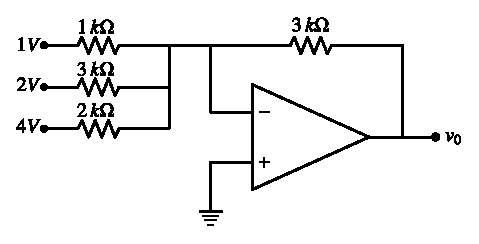
\includegraphics{chap4/figP4.24a.eps}

\smallskip
{\bf Fig. P4.25}
\end{figure}
\end{problem}

\begin{solution}
\begin{align*}
\rmV_{\rmo} &= -\left(\frac{\rmR_{\rmf}}{\rmR_{\rma}}\rmV_{1}+\frac{\rmR_{\rmf}}{\rmR_{\rmb}}\rmV_{2}+\frac{\rmR_{\rmf}}{\rmR_{\rmc}}\rmV_{3}\right)\\[3pt]
&= - \left(\frac{3}{1}\times 1+\frac{3}{3}\times 2+\frac{3}{2}\times 4\right)
\end{align*}
Output voltage $=\rmV_{\rmo}=-11$ V.
\end{solution}

\begin{problem}\label{prob4.26}
Find the output voltage in the circuit shown in Fig.~P4.26.
\begin{figure}[H]
\centering
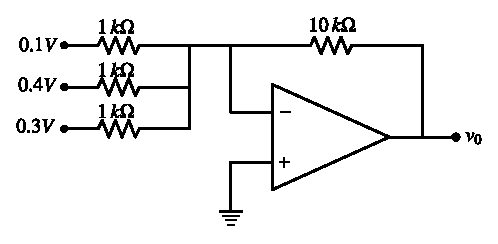
\includegraphics{chap4/figP4.25.eps}

\smallskip
{\bf Fig. P4.26}
\end{figure}
\end{problem}

\begin{solution}
\begin{align*}
&\rmR_{\rmf}=10\text{~k}\Omega,\quad \rmR_{\rma}=\rmR_{\rmb}=\rmR_{\rmc}=\rmR=1~\rmk\Omega\\[3pt]
&\rmV_{\rma}=0.1\rmV,\quad \rmV_{\rmb}=0.4\rmV,\quad \rmV_{\rmc}=0.3\rmV
\end{align*}
We have
\begin{align*}
\rmV_{\rmo} &= -\frac{\rmR_{\rmf}}{\rmR}(\rmV_{\rma}+\rmV_{\rmb}+\rmV_{\rmc})\\[3pt]
&= -\frac{10}{1}(0.1+0.4+0.3)
\end{align*}
$\therefore$~ Output voltage $\rmV_{\rmo}=-8\rmV$.
\end{solution}

\begin{problem}\label{prob4.27}
Design a summing amplifier to add three d.c. input voltages. The output of the circuit must be equal to two times the negative sum of the inputs.
\end{problem}

\begin{solution}
Let the three input voltages are $\rmV_{\rma}$, $\rmV_{\rmb}$ and $\rmV_{\rmc}$.

\medskip
The output voltage must be $\rmV_{\rmo}=-2(\rmV_{\rma}+\rmV_{\rmb}+\rmV_{\rmc})$

\medskip
We have 
\begin{align*}
\rmV_{\rmo} &=-\frac{\rmR_{\rmF}}{\rmR}(\rmV_{\rma}+\rmV_{\rmb}+\rmV_{\rmc})\\[3pt]
\therefore\quad \frac{\rmR_{\rmF}}{\rmR} &= 2
\end{align*}

Let $\rmR_{\rmF}=2~\rmk\Omega$ then, $\rmR=\dfrac{\rmR_{\rmF}}{2}=1~\rmk\Omega$

The designed circuit is shown in Fig.~P4.27.
\begin{figure}[H]
\centering
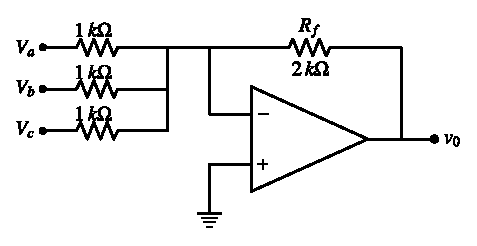
\includegraphics{chap4/figP4.26.eps}

\smallskip
{\bf Fig. P4.27}
\end{figure}
\end{solution}

\begin{problem}\label{prob4.28}
Design an adder circuit using an opamp to get the output expression as,
$$
\rmV_{\rmo}=-(0.1\rmV_{\rma}+\rmV_{\rmb}+10\rmV_{\rmc})
$$
where $\rmV_{\rma}$, $\rmV_{\rmb}$ and $\rmV_{\rmc}$ are inputs.
\end{problem}

\begin{solution}
We have $\rmV_{\rmo}=-\left(\dfrac{\rmR_{\rmf}}{\rmR_{\rma}}\rmV_{\rma}+\dfrac{\rmR_{\rmf}}{\rmR_{\rmb}}\rmV_{\rmb}+\dfrac{\rmR_{\rmf}}{\rmR_{\rmc}}\rmV_{\rmc}\right)$

\smallskip
Comparing with the given equation, we have
$$
\dfrac{\rmR_{\rmF}}{\rmR_{\rma}}=0.1,\quad \dfrac{\rmR_{\rmF}}{\rmR_{\rmb}}=1\quad\text{and}\quad \dfrac{\rmR_{\rmF}}{\rmR_{\rmc}}=10
$$

Let $\rmR_{\rmF}=10$~k$\Omega$, then we get,
$$
\rmR_{\rma}=100~\rmk\Omega,\quad \rmR_{\rmb}=10~\rmk\Omega\quad\text{and}\quad \rmR_{\rmc}=1~\rmk\Omega
$$

\eject

The circuit is shown in Fig.~P4.28.
\begin{figure}[H]
\centering
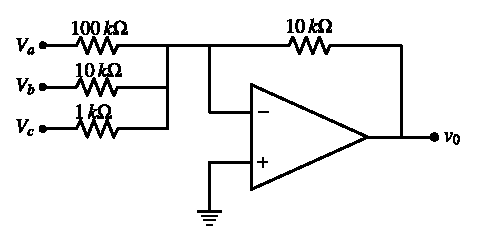
\includegraphics[scale=.95]{chap4/figP4.27.eps}

\smallskip
{\bf Fig. P4.28}
\end{figure}
\end{solution}

\begin{problem}\label{prob4.29}
\begin{itemize}
\item[(i)] Find the output voltage $\rmV_{\rmo}$ in Fig.~P4.29, if $\rmR_{\rmf}=10~\rmk\Omega$, $\rmR_{\rma}=2~\rmk\Omega$ and $\rmR_{\rmb}=5~\rmk\Omega$.

\item[(ii)] Find $\rmR_{\rma}$ and $\rmR_{\rmb}$, if $\rmV_{\rmo}$ is the average of $\rmV_{\rma}$ and $\rmV_{\rmb}$ with $\rmR_{\rmf}=10~\rmk\Omega$.
\begin{figure}[H]
\centering
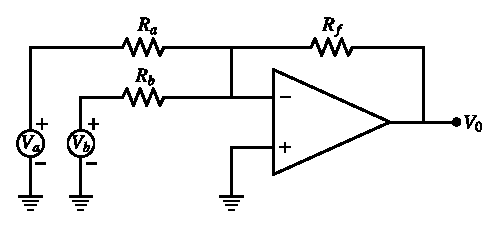
\includegraphics[scale=.95]{chap4/figP4.28.eps}

\smallskip
{\bf Fig. P4.29}
\end{figure}
\end{itemize}
\end{problem}

\begin{solution}
\begin{itemize}
\item[(i)] Given $\rmR_{\rmf}=10~\rmk\Omega$, \ $\rmR_{\rma}=2~\rmk\Omega$, \ $\rmR_{\rmb}=5~\rmk\Omega$

From the circuit we have,
\begin{align*}
\rmV_{\rmo} &= -\left(\frac{\rmR_{\rmf}}{\rmR_{\rma}}\rmV_{\rma}+\frac{\rmR_{\rmf}}{\rmR_{\rmb}}\rmV_{\rmb}\right)
= -\left(\frac{10}{2}\rmV_{\rma}+\frac{10}{5}\rmV_{\rmb}\right)
\end{align*}
Output voltage $\rmV_{\rma}=-(5\rmV_{\rma}+2\rmV_{\rmb})$

\item[(ii)] Given $\rmR_{\rmF}=10~\rmk\Omega$

\smallskip
The required output voltage 
\begin{align*}
\rmV_{\rmo} &=-\left(\dfrac{\rmV_{\rma}+\rmV_{\rmb}}{2}\right)\\[3pt]
\text{i.e.,}\quad \rmV_{\rmo} &=-\left(\frac{1}{2}\rmV_{\rmo}+\frac{1}{2}\rmV_{\rmb}\right)
\end{align*}

\vfill\eject

From the circuit we have $\rmV_{\rmo}=-\left(\dfrac{\rmR_{\rmf}}{\rmR_{\rma}}\rmV_{\rma}+\dfrac{\rmR_{\rmf}}{\rmR_{\rmb}}\rmV_{\rmb}\right)$

\medskip
By comparison \ $\dfrac{\rmR_{\rmF}}{\rmR_{\rma}}=\dfrac{\rmR_{\rmF}}{\rmR_{\rmb}}=\dfrac{1}{2}$

\medskip
$\therefore$~ Since $\rmR_{\rmF}=10~\rmk\Omega$, we get $\rmR_{\rma}=\rmR_{\rmb}=20~\rmk\Omega$.
\end{itemize}
\end{solution}

\begin{problem}\label{prob4.30}
Calculate $\rmV_{\rmo}$ for the circuit shown in Fig.~P4.30, if $\rmV_{1}=3\rmV$ and $\rmV_{2}=2\rmV$.
\begin{figure}[H]
\centering
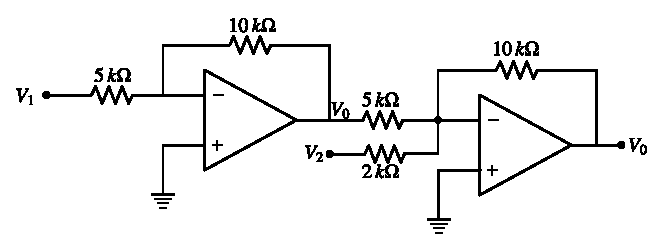
\includegraphics{chap4/figP4.29.eps}

\smallskip
{\bf Fig. P4.30}
\end{figure}
\end{problem}

\begin{solution}
Given $\rmV_{1}=3\rmV$; $\rmV_{2}=2\rmV$. In this given circuit there are two amplifiers cascaded in series. The first stage is an inverting amplifier and the second is summing amplifier or summer.

\smallskip
The output of first stage $\rmV_{\rmo}=-\dfrac{\rmR_{\rmf}}{\rmR_{1}}\rmV_{1}=-\dfrac{10}{5}\times 3=-6\rmV$ and $\rmV_{2}=2\rmV$.

\smallskip
$\therefore$~ The output voltage from the second stage is,
\begin{align*}
\rmV_{\rmo} &= -\left(\dfrac{10}{5}\rmV^{1}_{0}+\dfrac{10}{2}\rmV_{2}\right)\\[4pt]
&=-\left[\frac{10}{5}\times (-6)+\dfrac{10}{2}\times (2)\right]\\[4pt]
\rmV_{\rmo} &= 4\rmV
\end{align*}
\end{solution}

\itheading{Adder in Non-inverting configuration}~: If input voltage sources and resistors are connected to the non-inverting terminal of the opamp as shown in Fig.~\ref{fig4.11}, the circuit is called {\em non-inverting adder or summer}.
\begin{figure}[H]
\centering
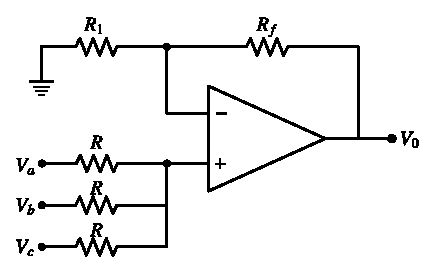
\includegraphics{chap4/fig4.11a.eps}
\caption{}\label{fig4.11}
\end{figure}

Since the input resistance of the non-inverting amplifier is very large, we can employ superposition theorem to obtain voltage at the non-inverting input terminal. 
\begin{align}
\text{i.e.,}\qquad \rmV_{1} &= \frac{\frac{\rmR}{2}}{\rmR+\frac{\rmR}{2}}\rmV_{\rma}+\frac{\frac{\rmR}{2}}{\rmR+\frac{\rmR}{2}}\rmV_{\rmb}+\frac{\frac{\rmR}{2}}{\rmR+\frac{\rmR}{2}}\rmV_{\rmc}\notag\\[5pt]
\rmV_{1} &= \frac{\rmV_{\rma}}{3}+\frac{\rmV_{\rmb}}{3}+\frac{\rmV_{c}}{3}\notag\\[5pt]
\rmV_{1} &= \frac{\rmV_{\rma}+\rmV_{\rmb}+\rmV_{\rmc}}{3}\label{eq4.34}
\end{align}
\begin{equation}
\therefore\quad \text{The output voltage~ } \rmV_{\rmo}=\left(1+\frac{\rmR_{\rmF}}{\rmR_{1}}\right)\rmV_{1}\label{eq4.35}
\end{equation}

Substituting Eqn.~\eqref{eq4.35} in Eqn.~\eqref{eq4.34}, we get
\begin{equation}
\rmV_{\rmo}=\left(1+\frac{\rmR_{\rmF}}{\rmR_{1}}\right)\left(\frac{\rmV_{\rma}+\rmV_{\rmb}+\rmV_{\rmc}}{3}\right)\label{eq4.36}
\end{equation}

Therefore the output voltage $\rmV_{\rmo}$ is equal to the average of all input voltages times the gain $\left(1+\dfrac{\rmR_{\rmF}}{\rmR_{1}}\right)$ of the circuit. Hence it is called an {\em average amplifier}.

If the gain $\left(1+\dfrac{\rmR_{\rmF}}{\rmR_{1}}\right)$ in Eqn.~\eqref{eq4.36} is equal to the number of inputs, the output voltage becomes equal to the sum of all input voltages. i.e., if $1+\dfrac{\rmR_{\rmF}}{\rmR_{1}}=3$, we get
\begin{equation}
\rmV_{\rmo}=\rmV_{\rma}+\rmV_{\rmb}+\rmV_{\rmc}\label{eq4.37}
\end{equation}

\eject

\begin{center}
\rule{4cm}{1pt}\\
{\bf\Large Problems}\\[-3pt]
\rule{4cm}{1pt}
\end{center}

\begin{problem}\label{prob4.31}
Determine the output voltage $\rmV_{\rmo}$ in the circuit shown in Fig.~P4.31.
\begin{figure}[H]
\centering
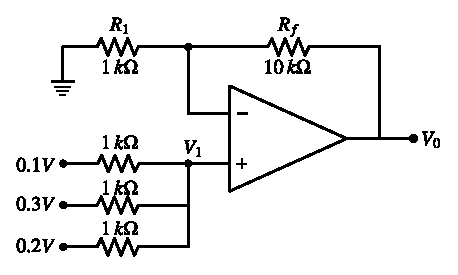
\includegraphics{chap4/figP4.30.eps}

\smallskip
{\bf Fig. P4.31}
\end{figure}
\end{problem}

\begin{solution}
The circuit is summer in non-inverting configuration. First, let us find voltage $\rmV_{1}$, at the non-inverting terminal using superposition theorem.
\begin{align*}
\rmV_{1} &= \frac{1\times 10^{3}}{1\times 10^{3}+\frac{1\times 10^{3}\times 1\times 10^{3}}{1\times 10^{3}+1\times 10^{3}}}\times 0.1+\frac{1\times 10^{3}}{1\times 10^{3}+\frac{1\times 10^{3}\times 1\times 10^{3}}{1\times 10^{3}+1\times 10^{3}}}\times 0.3\\[4pt]
&\hspace{4.7cm} +\dfrac{1\times 10^{3}}{1\times 10^{3}+\frac{1\times 10^{3}\times 1\times 10^{3}}{1\times 10^{3}+1\times 10^{3}}}\times 0.2\\[4pt]
\rmV_{1} &= 0.0667+0.2+0.1333\\[3pt]
\rmV_{1} &= 0.4\rmV
\end{align*}

We have closed loop gain \ $A_{v}=\dfrac{v_{\rmo}}{v_{\text{in}}}=\dfrac{v_{\rmo}}{v_{1}}=1+\dfrac{\rmR_{\rmf}}{\rmR_{1}}$.
\begin{align*}
\therefore\quad \text{Output voltage~ } \rmV_{\rmo} &= \left(1+\dfrac{\rmR_{\rmF}}{\rmR_{1}}\right)\rmV_{1}\\[4pt]
&= \left(1+\dfrac{10\times 10^{3}}{1\times 10^{3}}\right)\times 0.4\\[4pt]
\rmV_{\rmo} &= 4.4\rmV
\end{align*}
\end{solution}

\eject

\begin{problem}\label{prob4.32}
Determine the output voltage $\rmV_{\rmo}$ in the circuit shown in Fig.~P4.32.
\begin{figure}[H]
\centering
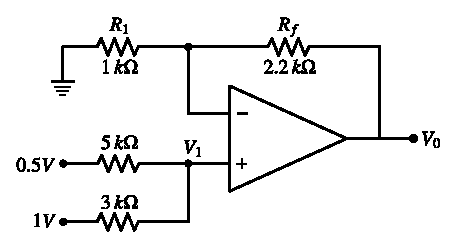
\includegraphics[scale=.95]{chap4/figP4.31.eps}

\smallskip
{\bf Fig. P4.32}
\end{figure}
\end{problem}

\begin{solution}
The given circuit is a summer in non-inverting configuration with two inputs. Applying superposition theorem at the non-inverting terminal, we get,
\begin{align*}
\rmV_{1} &= \frac{3\times 10^{3}}{5\times 10^{3}+3\times 10^{3}}\times 0.5 + \frac{5\times 10^{3}}{5\times 10^{3}+3\times 10^{3}}\times 1\\[4pt]
\rmV_{1} &= 0.1875+0.625\\[3pt]
\rmV_{1} &= 0.8125\rmV
\end{align*}
\vskip -.7cm
\begin{align*}
\therefore\quad \text{Output voltage~ } \rmV_{\rmo} &= \left(1+\frac{\rmR_{\rmF}}{\rmR_{1}}\right)\rmV_{1}
= \left(1+\frac{2.2\times 10^{3}}{1\times 10^{3}}\right)\times 0.8125\\[3pt]
\rmV_{\rmo} &= 2.6\rmV
\end{align*}
\end{solution}

\itheading{Subtractor~:}

A basic differential amplifier (i.e., inputs are applied to both inverting and non-inverting terminals) can be used as a {\em subtractor} as shown in Fig.~\ref{fig4.12}. If all resistors are equal, then the output voltage can be derived by using superposition principle.
\begin{figure}[H]
\centering
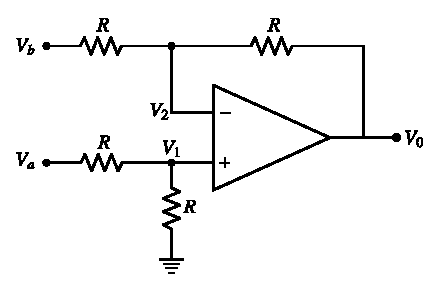
\includegraphics[scale=.95]{chap4/fig4.12.eps}
\caption{}\label{fig4.12}
\end{figure}

To find the output voltage $\rmV_{\rmo\rma}$ due to input $\rmV_{\rma}$ alone, make $\rmV_{\rmb}=0$. Then the circuit becomes non-inverting amplifier.
\begin{align}
\text{We have}\qquad \rmV_{1} &= \frac{\rmR}{\rmR+\rmR}\cdot \rmV_{\rma}\notag\\[4pt]
\rmV_{1} &= \frac{1}{2}\rmV_{\rma}\label{eq4.38}\\[3pt]
\therefore\quad \rmV_{\rmo\rma} &= \left(1+\dfrac{\rmR}{\rmR}\right)\rmV_{1}\notag\\[3pt]
\rmV_{\rmo\rma} &= 2\rmV_{1}\label{eq4.39}
\end{align}

Substituting Eqn.~\eqref{eq4.38} in Eqn.~\eqref{eq4.39}, we get,
\begin{align}
\rmV_{\rmo\rma} &= 2\cdot \frac{1}{2}\cdot \rmV_{\rma}\notag\\[3pt]
\therefore\quad \rmV_{\rmo\rma} &= \rmV_{\rma}\label{eq4.40}
\end{align}

Similarly, to find the output voltage $\rmV_{\rmo\rmb}$ due to $\rmV_{\rmb}$ alone, make $\rmV_{\rma}=0$. Then the circuit becomes inverting amplifier with gain $-\rmR/\rmR=-1$.
\begin{align}
\therefore\quad \rmV_{\rmo\rmb} &= -\frac{\rmR}{\rmR}\cdot \rmV_{\rmb}\notag\\[3pt]
\rmV_{\rmo\rmb} &= -\rmV_{\rmb}\label{eq4.41}
\end{align}

Thus, the total output voltage,
\begin{equation}
\rmV_{\rmo}=\rmV_{\rmo\rma}+\rmV_{\rmo\rmb}\label{eq4.42}
\end{equation}

Substituting Eqns.~\eqref{eq4.40} and \eqref{eq4.41} in Eqn.~\eqref{eq4.42},
\begin{equation}
\therefore\quad \rmV_{\rmo}=\rmV_{\rma}-\rmV_{\rmb}\label{eq4.43}
\end{equation}

Thus, the output voltage $\rmV_{\rmo}$ is equal to the voltage $\rmV_{\rma}$ applied to the non-inverting terminal minus the voltage $\rmV_{\rmb}$ applied to the inverting terminal. Therefore the circuit is called as {\em subtractor}.

\eject

\begin{center}
\rule{4cm}{1pt}\\
{\bf\Large Problems}\\[-3pt]
\rule{4cm}{1pt}
\end{center}

\begin{problem}\label{prob4.33}
In the subtractor circuit shown in Fig.~P4.33, determine the output voltage.
\begin{figure}[H]
\centering
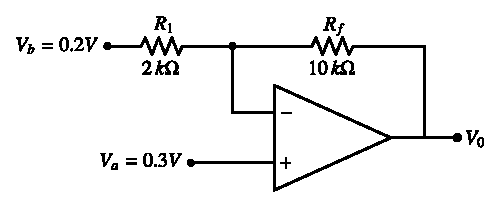
\includegraphics{chap4/figP4.32.eps}

\smallskip
{\bf Fig. P4.33}
\end{figure}
\end{problem}

\begin{solution}
The output voltage can be found using superposition theorem as before. To find the output voltage $\rmV_{\rmo\rma}$ due to the input $\rmV_{\rma}$ only, make $\rmV_{\rmb}=0$.
\begin{align*}
\rmV_{\rmo\rma} &= \left(1+\frac{10\times 10^{3}}{2\times 10^{3}}\right)\times 0.3\\[4pt]
\rmV_{\rmo\rma} &= 1.8\rmV
\end{align*}

To find the output voltage $\rmV_{\rmo\rmb}$ due to the input $\rmV_{\rmb}$ only, make $\rmV_{\rma}=0$
\begin{align*}
\rmV_{\rmo\rmb} &= -\frac{10\times 10^{3}}{2\times 10^{3}}\times 0.2\\[3pt]
\rmV_{\rmo\rmb} &= -1\rmV
\end{align*}
$\therefore$~ The total output voltage 
\begin{align*}
\rmV_{\rmo} &= \rmV_{\rmo\rma}+\rmV_{\rmo\rmb}\\[3pt]
&= 1.8-1\\[3pt]
\rmV_{\rmo} &= 0.8\rmV
\end{align*}
\end{solution}

\eject

\begin{problem}\label{prob4.34}
Find the output voltage in the circuit shown in Fig.~P4.34.
\begin{figure}[H]
\centering
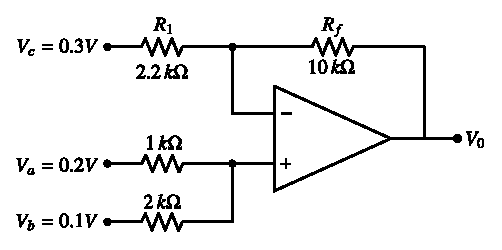
\includegraphics[scale=.96]{chap4/figP4.33.eps}

\smallskip
{\bf Fig. P4.34}
\end{figure}
\end{problem}

\begin{solution}
The output voltage can be obtained by using superposition theorem as below. 

\smallskip
To find the output voltage $\rmV_{\rmo\rma}$ due to input $\rmV_{\rma}$ alone, make $\rmV_{\rmb}=\rmV_{\rmc}=0$.

\smallskip
Then the circuit becomes as shown in Fig.~P4.34.1.
\begin{figure}[H]
\centering
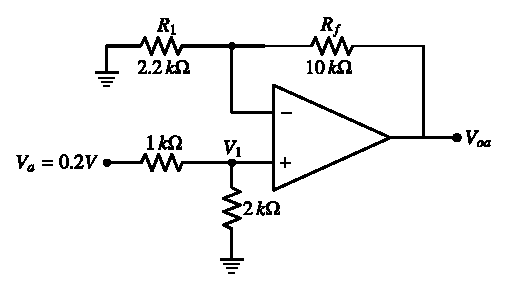
\includegraphics[scale=.96]{chap4/figP4.33.1.eps}

\smallskip
{\bf Fig. P4.34.1}
\end{figure}

From Fig.~P4.34.1,
\begin{align*}
\rmV_{1} &= \frac{2\times 10^{3}}{1\times 10^{3}+2\times 10^{3}}\rmV_{\rma}= 0.667\times 0.2\\[3pt]
\rmV_{1} &= 0.1334\rmV\\[3pt]
\therefore\quad \rmV_{\rmo\rma} &= \left(1+\frac{\rmR_{\rmF}}{\rmR_{1}}\right)\rmV_{1}\\[3pt]
&= \left(1+\frac{10\times 10^{3}}{2.2\times 10^{3}}\right)\times 0.1334\\[3pt]
&= 0.7398\rmV
\end{align*}

To find the output voltage $\rmV_{\rmo\rmb}$ due to input $\rmV_{\rmb}$ only, make $\rmV_{\rma}=\rmV_{\rmc}=0$. Then the circuit becomes as shown in Fig.~P4.33.2.
\begin{figure}[H]
\centering
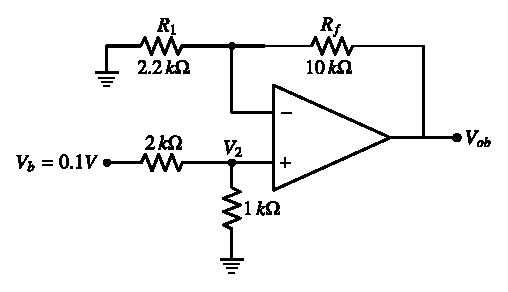
\includegraphics{chap4/figP4.33.2.eps}

\smallskip
{\bf Fig. P4.34.2}
\end{figure}

From Fig.~P4.34.2,
\begin{align*}
\rmV_{2} &= \frac{1\times 10^{3}}{1\times 10^{3}+2\times 10^{3}}\times \rmV_{\rmb}\\[4pt]
&= 0.333\times 0.1\\[4pt]
\rmV_{2} &= 0.0333\rmV\\[4pt]
\therefore\quad \rmV_{\rmo\rmb} &= \left(1+\frac{\rmR_{\rmF}}{\rmR_{1}}\right)\rmV_{2}\\[4pt]
&= \left(1+\frac{10\times 10^{3}}{2.2\times 10^{3}}\right)\times 0.0333\\[3pt]
\rmV_{\rmo\rmb} &= 0.1847\rmV
\end{align*}
To find the output voltage $\rmV_{\rmo\rmc}$ due to input $\rmV_{\rmc}$ only, make $\rmV_{\rma}=\rmV_{\rmb}=0$. Then the circuit becomes as shown in Fig.~P4.34.3.
\begin{figure}[H]
\centering
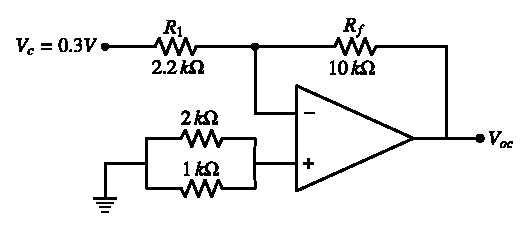
\includegraphics{chap4/figP4.33.3.eps}

\smallskip
{\bf Fig. P4.34.3}
\end{figure}

From Fig.~P4.34.3, 
\begin{align*}
\rmV_{\rmo\rmc} &= -\frac{\rmR_{\rmF}}{\rmR_{1}}\rmV_{\rmc}\\[4pt]
&= -\frac{10\times 10^{3}}{2.2\times 10^{3}}\times 0.3\\[4pt]
\rmV_{\rmo\rmc} &=-1.364\rmV
\end{align*}
$\therefore$~ The total output voltage 
\begin{align*}
\rmV_{\rmo} &= \rmV_{\rmo\rma}+\rmV_{\rmo\rmb}+\rmV_{\rmo\rmc}\\[4pt]
          &= 0.7398+0.1847-1.364\\[4pt]
\rmV_{\rmo} &= -0.4395\rmV
\end{align*}
\end{solution}

\subsection{Opamp Integrating Circuit ({\em Integrator})}\label{sec4.6.5}

An {\em integrator} is a circuit in which the output voltage is the integral of the input voltage. Fig.~\ref{fig4.13} shows an integrator circuit using opamp. The integrator may be constructed from a basic inverting amplifier if feedback resistor $\rmR_{\rmF}$ is replaced by a capacitor $\rmC_{\rmF}$.
\begin{figure}[H]
\centering
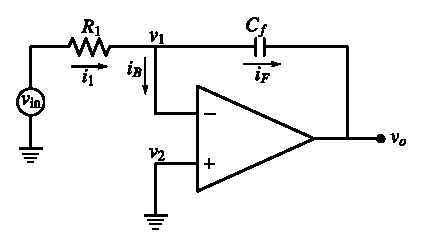
\includegraphics{chap4/fig4.13.eps}
\caption{Basic integrator circuit}\label{fig4.13}
\end{figure}

Applying KCL at node $v_{1}$,
\begin{align}
\rmi_{1} &= \rmi_{\rmB}+\rmi_{\rmF}\label{eq4.44}\\[4pt]
\rmi_{1} &\simeq \rmi_{\rmF}\quad (\because \ \rmi_{\rmB}=0)\label{eq4.45}
\end{align}

\eject

We know that current through a capacitor is given by
\begin{equation}
\rmi_{\rmc} = \rmC\frac{\rmd v_{\rmc}}{\dt}\label{eq4.46}
\end{equation}
where $v_{\rmc}$ is voltage across the capacitor.

$\therefore$~ From Eqn.~\eqref{eq4.45} and \eqref{eq4.46},
\begin{equation}
\frac{v_{\text{in}}-v_{2}}{\rmR_{1}}=\rmC_{\rmF}\dfrac{\rmd (v_{2}-v_{\rmo})}{\dt}\label{eq4.47}
\end{equation}

But\quad $v_{\text{id}}\simeq v_{2}-v_{1}=0$\quad $\therefore~ v_{1}\simeq v_{2}\simeq 0$

$\therefore$~ From Eqn.~\eqref{eq4.47},
\begin{equation}
\frac{v_{\text{in}}}{\rmR_{1}}=\rmC_{\rmF}\frac{\rmd}{\dt}(-v_{\rmo})\label{eq4.48}
\end{equation}

Integrating Eqn.~\eqref{eq4.48} with respect time,
\begin{align}
\int\limits^{t}_{0}\frac{v_{\text{in}}}{\rmR_{1}}\dt &= \int\limits^{t}_{0}\rmC_{\rmF}\dfrac{\rmd}{\dt}(-v_{\rmo})\dt\notag\\[3pt]
\int\limits^{t}_{0}\dfrac{\rmd v_{\rmo}}{\dt} &= -\dfrac{1}{\rmR_{1}\rmC_{\rmF}}\int\limits^{t}_{0}v_{\text{in}}\dt\notag\\[3pt]
v_{\rmo} &= -\frac{1}{\rmR_{1}\rmC_{\rmF}}\int\limits^{\rmt}_{0}v_{\text{in}}\dt+\rmC\label{eq4.49}
\end{align}
where $\rmC$ is the integration constant and is proportional to the value of the output voltage $v_{\rmo}$ at time $\rmt=0$ sec. From Eqn.~\eqref{eq4.49}, it is observed that the output voltage is directly proportional to the negative integral of the input voltage and inversely proportional to the time constant $\rmR_{1}\rmC_{\rmF}$.

\begin{center}
\rule{4cm}{1pt}\\
{\bf\Large Problems}\\[-3pt]
\rule{4cm}{1pt}
\end{center}

\begin{problem}\label{prob4.35}
In the circuit shown in Fig.~P4.35, the input is a step (dc) voltage as shown in Fig.~P4.35.1. Determine the output voltage and sketch it. Assume that the initial voltage across capacitor is zero. Time constant $\rmR_{1}\rmC_{\rmF}=1$ second.
\begin{figure}[H]
\centering
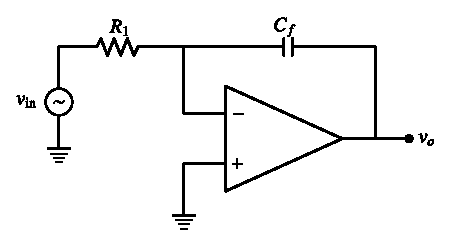
\includegraphics{chap4/figP4.34.eps}

\smallskip
{\bf Fig. P4.35}
\end{figure}
\begin{figure}[H]
\centering
\includegraphics{chap4/figP4.34.1.eps}

\smallskip
{\bf Fig. P4.35.1}
\end{figure}
\end{problem}

\begin{solution}
Given $\rmR_{1}\rmC_{\rmF}=1$~sec.
\smallskip

The input is constant, 3V for $0\leq \rmt\leq 5$ sec. The given circuit is an ideal integrator. The output voltage is given by,
\begin{align*}
\rmv_{\rmo} &= -\frac{1}{\rmR_{1}\rmC_{\rmF}}\int\limits^{\rmt}_{0}v_{\text{in}}\dt\\[3pt]
&= -\int\limits^{\rmt}_{0}3\,\dt\\[3pt]
v_{\rmo} &= -3\rmt \ \rmV
\end{align*}

The output voltage $v_{\rmo}$ is sketched in Fig.~P4.35.2.
\begin{figure}[H]
\centering
\includegraphics{chap4/figP4.34.2.eps}

\smallskip
{\bf Fig. P4.35.2}
\end{figure}
\end{solution}

\begin{problem}\label{prob4.36}
A sinusoidal signal with peak value 6mV and of 2\,kHz is applied to the input of an ideal opamp integrator with $\rmR_{1}=100\,\rmk\Omega$ and $\rmC_{\rmF}=1\,\mu\rmF$. Find the output voltage.
\end{problem}

\begin{solution}
Given $\rmR_{1}=100\,\rmk\Omega$, \ $\rmC_{\rmF}=1\,\mu\rmF$, \ $\rmV_{\max}=6$\,mV, \ $\rmf=2$\,kHz.

We know that the output voltage is given by
$$
v_{\rmo}=-\frac{1}{\rmR_{1}\rmC_{\rmF}}\int\limits^{\rmt}_{0}v_{\text{in}}+\rmC
$$
where C = initial voltage across the capacitor. Assuming C = 0,
\begin{align*}
v_{\rmo} &= -\frac{1}{100\times 10^{3}\times 1\times 10^{-6}}\int\limits^{\rmt}_{0}6\sin 4000 \pi\,\rmt\quad [\because \ \omega=2\pi\rmf=4000\pi]\\[3pt]
&=-60\left[-\frac{\cos 4000\pi \rmt}{4000\pi}\right]^{\rmt}_{0}\\[3pt]
v_{\rmo} &= \frac{0.015}{\pi}[\cos 4000 \pi\rmt-1]\text{~mV}
\end{align*}
\end{solution}

\begin{problem}\label{prob4.37}
Determine and sketch the output voltage waveform if an input voltage shown in Fig.~P4.37 is applied to an ideal integrator. Assume time constant $\rmR_{1}\rmC_{\rmF}=1$ second and initial voltage across capacitor = 0 V.
\begin{figure}[H]
\centering
\includegraphics{chap4/figP4.36.eps}

\smallskip
{\bf Fig. P4.37}
\end{figure}
\end{problem}

\begin{solution}
The output voltage waveform is sketched in Fig.~P4.37.1.
\begin{figure}[H]
\centering
\includegraphics{chap4/figP4.36.1.eps}

\smallskip
{\bf Fig. P4.37.1}
\end{figure}
\end{solution}

\begin{problem}\label{prob4.38}
In an ideal integrator circuit, the input is a sine wave with peak-to-peak amplitude of 5V at 1\,kHz. Find the output voltage, if $\rmR_{1}\rmC_{\rmF}=0.1$ ms. Assume that the voltage across $\rmC_{\rmF}$ is initially zero.
\end{problem}

\begin{solution}
Given \ $\rmR_{1}\rmC_{\rmF}=0.1$\, ms.
$$
\omega =2\pi \rmf=2\times \pi\times 1\times 10^{3}\simeq 6283\text{~rad/sec.}
$$
$\therefore$~ $v_{\text{in}}=2.5\sin 6283\,\rmt$.

We have,
\begin{align*}
v_{\rmo} &= -\frac{1}{\rmR_{1}\rmC_{\rmF}}\int\limits^{\rmt}_{0}v_{\text{in}}\dt +\rmC\\
v_{\rmo} &= -\frac{1}{0.1\times 10^{-3}}\int\limits^{\rmt}_{0}2.5\sin 6283\,\rmt\,\dt\qquad [\because \ \rmC =0]\\
&=-25\times 10^{3}\left[-\frac{\cos 6283\rmt}{6283}\right]^{\rmt}_{0}\\
v_{\rmo} &= 3.98[\cos 6283\,\rmt-1]\rmV
\end{align*}
\end{solution}

\vfill\eject

\begin{problem}\label{prob4.39}
Determine the rate of change of the output voltage in response to the step input as shown in Fig.~P4.39 to an ideal integrator with time constant = 1.12 msec.
\begin{figure}[H]
\centering
\includegraphics{chap4/figP4.38.eps}

\smallskip
{\bf Fig. P4.39}
\end{figure}
\end{problem}

\begin{solution}
Time constant $\rmR_{1}\rmC_{\rmF}=1.12$ msec. and $\rmC=0$, $v_{\text{in}}=5\rmV$.

\medskip
We have \ $v_{\rmo}=-\dfrac{1}{\rmR_{1}\rmC_{\rmF}}\int v_{\text{in}}\dt +\rmC$.

\medskip
Differentiating with respect to time, we get
\begin{align*}
\dfrac{\rmd v_{\rmo}}{\dt} &= -\frac{v_{\text{in}}}{\rmR_{1}\rmC_{\rmF}}
= -\dfrac{5}{1.12\times 10^{-3}}\\[3pt]
\dfrac{\rmd v_{\rmo}}{\dt} &= -4464\text{~V/s.}\simeq -4.464\text{~mV}/\mu\rms.
\end{align*}
$\therefore$~ The rate of change of output voltage is 4.464 mV/$\mu$s.
\end{solution}

\subsection{Opamp Differentiating Circuit ({\em Differentiator})}\label{sec4.6.6}

A {\em differentiator} is a circuit in which the output voltage is the time derivative of the input voltage. Fig.~\ref{fig4.14} shows a differentiator circuit using opamp. The differentiator may be constructed from a basic inverting amplifier if an input resistor $\rmR_{1}$ is replaced by a capacitor $\rmC_{1}$.
\begin{figure}[H]
\centering
\includegraphics{chap4/fig4.14.eps}
\caption{Basic differentiator circuit}\label{fig4.14}
\end{figure}

\eject

Applying KCL at node $v_{1}$,
\begin{align}
\rmi_{\rmC} &= \rmi_{\rmB}+\rmi_{\rmF}\notag\\[3pt]
\therefore\quad \rmi_{\rmC} &\simeq \rmi_{\rmF}\label{eq4.50}
\end{align}
\begin{align}
\text{i.e.,}\quad \rmC_{1}\dfrac{\rmd (v_{\text{in}}-v_{1})}{\dt} &= \frac{v_{1}-v_{\rmo}}{\rmR_{\rmF}}\notag\\[3pt]
\rmC_{1}\dfrac{\rmd v_{\text{in}}}{\dt} &=\frac{-v_{\rmo}}{\rmR_{\rmF}}\qquad [\because \ v_{1}\simeq v_{2}=0]\notag\\[3pt]
\therefore\quad v_{\rmo} &= -\rmR_{\rmf}\rmC_{1}\dfrac{\rmd v_{\text{in}}}{\dt}\label{eq4.51}
\end{align}

Thus, the output voltage $v_{\rmo}$ is equal to $\rmR_{\rmF}\rmC_{1}$ (time constant) times the negative instantaneous rate of change of the input voltage $v_{\text{in}}$ with respect to time.

\begin{center}
\rule{4cm}{1pt}\\
{\bf\Large Problems}\\[-3pt]
\rule{4cm}{1pt}
\end{center}

\begin{problem}\label{prob4.40}
The input to a basic differentiator circuit is a sinusoidal voltage of peak value of 10 mV and frequency 1.5 kHz. Find the output if $\rmR_{\rmf}=100\,\rmk\Omega$ and $\rmC_{1}=1\,\mu\rmF$.
\end{problem}

\begin{solution}
Given $\rmR_{\rmF}=100\,\rmk\Omega$, \ $\rmC_{1}=1\mu\rmF$,  \ $v_{\text{in}}=10\sin 3000 \pi\rmt$ mV.

\medskip
Time constant $\rmR_{\rmF}\rmC_{1}=(100\times 10^{3})(1\times 10^{-6})=0.1$ sec.

\medskip
We have,
\begin{align*}
v_{0} &= -\rmR_{\rmF}\rmC_{1}\dfrac{\rmd v_{\text{in}}}{\dt}\\[3pt]
&= -0.1\dfrac{\rmd}{\dt}(10\sin 3000 \pi t)\\[3pt]
&= -0.1\times 10\times 3000 \pi \times \cos 3000\, \pi\, \rmt\\[3pt]
v_{\rmo} &= -3000\pi \cos 3000\, \pi\,\rmt \text{~ mV.}
\end{align*}
\end{solution}

\eject

\begin{problem}\label{prob4.41}
The input voltage waveform shown in Fig.~P4.40 is applied to a basic differentiator circuit with $\rmR_{\rmF}=1.5\,\rmk\Omega$ and $\rmC_{1}=0.1\,\mu\rmF$. Draw the output voltage waveform.
\begin{figure}[H]
\centering
\includegraphics[scale=.95]{chap4/figP4.40.eps}

\smallskip
{\bf Fig. P4.41}
\end{figure}
\end{problem}

\begin{solution}
Given~ $\rmR_{\rmF}=1.5\,\rmk\Omega$, \ $\rmC_{1}=0.1\,\mu\rmF$.

\medskip
$\therefore$~ Time constant $\rmR_{\rmF}\rmC_{1}=1.5\times 10^{3}\times 0.1\times 10^{-6}=0.15$ msec.

\medskip
From the given input voltage waveform,
$$
\rmT=1\text{~msec}\quad \therefore\quad f=\dfrac{1}{\rmT}=1\text{~kHz}
$$
\vskip -.7cm
\begin{align*}
\therefore\quad \omega &= 2\pi\rmf =2\pi\times 1000=2000\,\pi\text{~rad/sec.}\\[3pt]
\therefore\quad v_{\text{in}} &= 2\sin 2000\,\pi\, \rmt\\[3pt]
\text{We have~~ } v_{0} &= -\rmR_{\rmF}\rmC_{1}\dfrac{\rmd v_{\text{in}}}{\dt}\\[3pt]
&= -0.15\times 10^{-3}\times \dfrac{\rmd}{\dt}[2\sin 2000\,\pi\,\rmt]\\[3pt]
&= -0.15\times 10^{-3}\times 2\times 2000\,\pi\,\cos 2000\,\pi\,\rmt\\[3pt]
\therefore\quad v_{\rmo} &= -1.885\cos 2000\,\pi\,\rmt\;\rmV
\end{align*}
The output voltage waveform is plotted in Fig.~P4.41.1.
\begin{figure}[H]
\centering
\includegraphics[scale=.95]{chap4/figP4.40.1.eps}

\smallskip
{\bf Fig. P4.41.1~: Illustrating the problem 4.41}
\end{figure}
\end{solution}

\vfill\eject

\begin{problem}\label{prob4.42}
In a basic differentiator circuit, the input is a sine wave with a peak-to-peak amplitude of 3V at 200 Hz. Determine the output voltage. Given : time constant $\rmR_{\rmF}\rmC_{1}=0.15$ msec.
\end{problem}

\begin{solution}
Given \ $\rmR_{\rmF}\rmC_{1}=0.15$ msec, \ $\rmf=200$ Hz.
\begin{align*}
\omega &= 2\pi \rmf = 2\pi \times 200=400 \pi\text{~ rad/sec.}\\[3pt]
\therefore\quad v_{\text{in}} &= 1.5\sin 400 \pi \rmt\;\rmV
\end{align*}
We have
\begin{align*}
v_{\rmo} &= -\rmR_{\rmF}\rmC_{1}\dfrac{\rmd v_{\text{in}}}{\dt}\\[3pt]
&= -0.15\times 10^{-3}\dfrac{\rmd}{\dt}[1.5\sin 400 \pi \rmt]\\[3pt]
&= -0.15\times 10^{-3}\times 1.5\times 400\pi\,\cos 400 \,\pi \rmt
\end{align*}
$\therefore$~ Output voltage $v_{\rmo}=-0.283\cos 400\,\pi\rmt \ \rmV$.
\end{solution}

\begin{problem}\label{prob4.43}
Determine the output voltage of a basic opamp differentiator for the triangular-wave input shown in Fig.~P4.43. Given that the time constant $\rmR_{\rmF}\rmC_{1}=2.2\,\mu\rms$.
\begin{figure}[H]
\centering
\includegraphics{chap4/figP4.42.eps}

\smallskip
{\bf Fig. P4.43}
\end{figure}
\end{problem}

\begin{solution}
Given \ $\rmR_{\rmF}\rmC_{1}=2.2\,\mu\rms$.

\medskip
For $0<\rmt<5\,\mu\rms$, the rate of change of input voltage
\begin{align*}
\dfrac{\rmd v_{\text{in}}}{\dt} &= \frac{5-(-5)}{5\mu\rms}=2\rmV/\mu\rms\\[3pt]
\therefore\quad v_{\rmo} &= -\rmR_{\rmF}\rmC_{1}\dfrac{\rmd v_{\text{in}}}{\dt}\\[3pt]
&= -2.2\mu\rms \times \dfrac{2\rmV}{\mu\rms}\\[3pt]
&= -4.4\rmV
\end{align*}
For~ $5\mu\rms <\rmt < 10\mu\rms$, \ $\dfrac{\rmd v_{\text{in}}}{\dt}=\dfrac{-5-5\rmV}{5\,\mu\rms}=-2\rmV/\mu\rms$.
\begin{align*}
\therefore\quad v_{\rmo} &= -\rmR_{\rmF}\rmC_{1}\dfrac{\rmd v_{\text{in}}}{\dt}\\[3pt]
&= -2.2\mu\rms \times (-2\rmV/\mu\rms)\\[3pt]
v_{\rmo} &= 4.4\,\rmV
\end{align*}
These values repeats for every $10\,\mu\rms$.

The output voltage waveform is plotted relative to the input in Fig.~P4.43.1.
\begin{figure}[H]
\centering
\includegraphics{chap4/figP4.42.1.eps}

\smallskip
{\bf Fig. P4.43.1}
\end{figure}
\end{solution}

\begin{center}
\rule{4cm}{1pt}\\
{\bf\Large Exercises}\\[-3pt]
\rule{4cm}{1pt}
\end{center}

\begin{enumerate}
\renewcommand{\labelenumi}{(\theenumi)}
\item Determine the input bias current and input offset current to an opamp if the current into non-inverting and inverting terminals are $10\,\mu\rmA$ and $12.5\,\mu\rmA$ respectively.

\smallskip
\noindent
{\bf Ans~:} $\rmI_{\rmB}=11.25\,\mu\rmA$, \ $\rmI_{\text{io}}=2.5\,\mu\rmA$.

\item An opamp has a differential voltage gain of 1,55,000 and common-mode gain of 1.5. Determine the CMRR and express it in decibels.

\smallskip
\noindent
{\bf Ans~:} CMRR $\simeq$ 103333 $\simeq$ 100.3 dB

\item An opamp has a differential gain of 2800 and CMRR of 25,000.
\begin{itemize}
\item[(a)] Determine the common-mode gain.

\item[(b)] Express the CMRR in dB.
\end{itemize}

\smallskip
\noindent
{\bf Ans~:} (a)~ $\rmA_{\text{cm}}=0.112$\quad (b)~ CMRR = 87.96 dB

\item When a pulse is applied to an opamp, the output voltage goes from $-10\rmV$ to $+5\rmV$ in $1\,\mu\rms$. What is the slew rate ?

\smallskip
\noindent
{\bf Ans~:} 15 V/$\mu$s.

\item An opamp has a common input signal of 4\,V to both terminals. This results in an output signal of 25\,mV. Determine the common mode gain and the CMRR. Given that differential gain is 140.

\smallskip
\noindent
{\bf Ans~:} $\rmA_{\text{cm}}6.25\times 10^{-3}$, \ CMRR = 22,400 = 87 dB.

\item For the circuit of inverting amplifier with $\rmR_{\rmf}=470\,\rmk\Omega$ and $\rmR_{1}=2.2\,\rmk$, if $v_{\text{in}}=0.5\rmV$, Calculate,
\begin{itemize}
\item[(i)] Closed-loop gain

\item[(ii)] Output voltage
\end{itemize}

\item For the circuit of non-inverting amplifier with $\rmR_{\rmf}=470$\,k$\Omega$ and $\rmR_{1}=10\,\rmk\Omega$, if $v_{\text{in}}=1$ mV, calculate
\begin{itemize}
\item[(i)] closed loop gain

\item[(ii)] output voltage
\end{itemize}

\smallskip
\noindent
{\bf Ans~:} (i)~ $\rmA_{\rmf}=48$\quad (ii)~ $v_{\rmo}=48$\,mV.

\eject

\item Find the output voltage in the circuit shown below.
\begin{figure}[H]
\centering
\includegraphics{chap4/exr4.8.eps}
\end{figure}

\smallskip
\noindent
{\bf Ans~:} $v_{\rmo}=-9.88\,\rmV$.

\item Determine the output voltage in the circuit shown below.
\begin{figure}[H]
\centering
\includegraphics{chap4/exr4.9.eps}
\end{figure}

\smallskip
\noindent
{\bf Ans~:} $v_{\rmo}=1.86\,\rmV$.

\item In an ideal integrator circuit, the input is a sine wave with peak-to-peak amplitude of 8\,V at 1.5\,kHz. Find the output voltage if $\rmR_{1}\rmC_{\rmF}=0.18$ msec. Assume that the voltage across $\rmC_{\rmF}$ is initially zero.

\smallskip
\noindent
{\bf Ans~:} $v_{\rmo}=2.4[\cos 9425\rmt-1]\rmV$.
\end{enumerate}


\label{4end}
